% **************************************************
% Clean Thesis
% -- A LaTeX Style for Thesis Documents --
%
% Copyright (C) 2011-2015 Ricardo Langner
% **************************************************
%
% Readme:
% ----------------------------------------
% Please check out the README.md file in the root of this package.
%
%
% License Information:
% ----------------------------------------
% "Clean Thesis" is free software: you can redistribute it and/or modify
% it under the terms of the GNU General Public License as published by
% the Free Software Foundation, either version 3 of the License, or
% (at your option) any later version.
%
% "Clean Thesis" is distributed in the hope that it will be useful,
% but WITHOUT ANY WARRANTY; without even the implied warranty of
% MERCHANTABILITY or FITNESS FOR A PARTICULAR PURPOSE.  See the
% GNU General Public License for more details.
%
% You should have received a copy of the GNU General Public License
% along with this program.  If not, see <http://www.gnu.org/licenses/>.
% **************************************************

%\newcommand{\LeDraft}{true}
\newcommand{\LeDraft}{false}

% **************************************************
% Document Class Definition
% **************************************************
\documentclass[%
	paper=A4,					% paper size --> A4 is default in Germany
	twoside=true,				% onesite or twoside printing
	openright,					% doublepage cleaning ends up right side
	parskip=full,				% spacing value / method for paragraphs
	chapterprefix=true,			% prefix for chapter marks
	10pt,						% font size
	headings=normal,			% size of headings
	bibliography=totoc,			% include bib in toc
	listof=totoc,				% include listof entries in toc
	titlepage=on,				% own page for each title page
	captions=tableabove,		% display table captions above the float env
	draft=\LeDraft,				% value for draft version
]{scrreprt}%

% **************************************************
% Debug LaTeX Information
% **************************************************
%\listfiles

% **************************************************
% Load and Configure Packages
% **************************************************
\usepackage[T1]{fontenc}
\usepackage[utf8]{inputenc}
\usepackage{lmodern}

% **************************************************
% Information and Commands for Reuse
% **************************************************
\newcommand{\thesisTitle}{Personal Perception and Interaction in Mixed Reality}
\newcommand{\thesisName}{Meng Ma}
\newcommand{\thesisSubject}{Dissertation}
\newcommand{\thesisDate}{\today}
\newcommand{\thesisVersion}{0.0}

\newcommand{\thesisVorsitzender}{...}
\newcommand{\thesisVorsitzenderAffiliation}{...}

\newcommand{\thesisFirstReviewer}{Prof. Nassir Navab, Ph.D.}
\newcommand{\thesisFirstReviewerAffiliation}{
	Technische Universität München\\[-1mm]
	Computer Aided Medical Procedures
}

\newcommand{\thesisSecondReviewer}{\TODO{Prof. Dr.-Ing. Bernhard Preim}}
\newcommand{\thesisSecondReviewerAffiliation}{
	 Otto-von-Guericke-Universität\\[-1mm]
	 Institut für Simulation und Graphik
}

\newcommand{\thesisFirstSupervisor}{Prof. Nassir Navab}
\newcommand{\thesisSecondSupervisor}{Dr. Maximilian Baust}

\newcommand{\thesisUniversity}{\protect{Technische Universität München}}
\newcommand{\thesisUniversityDepartment}{Fakultät für Informatik}
\newcommand{\thesisUniversityInstitute}{Lehrstuhl für Informatikanwendungen in der Medizin \& Augmented Reality}
\newcommand{\thesisUniversityGroup}{}
\newcommand{\thesisUniversityCity}{Garching bei München}
\newcommand{\thesisUniversityStreetAddress}{Boltzmannstraße 3}
\newcommand{\thesisUniversityPostalCode}{85748}


% **************************************************
% Load and Configure Packages
% **************************************************
\usepackage[english]{babel} 	% babel system, adjust the language of the content
\usepackage[					% clean thesis style
	figuresep=colon,%
	sansserif=false,%
	hangfigurecaption=true,%
	hangsection=true,%
	hangsubsection=true,%
	colorize=full,%
	colortheme=bluemagenta,
	draft=\LeDraft				% value for draft version
]{cleanthesis}

\hypersetup{					% setup the hyperref-package options
	pdftitle={\thesisTitle},	% 	- title (PDF meta)
	pdfsubject={\thesisSubject},% 	- subject (PDF meta)
	pdfauthor={\thesisName},	% 	- author (PDF meta)
	plainpages=false,			% 	-
	colorlinks=false,			% 	- colorize links?
	pdfborder={0 0 0},			% 	-
	breaklinks=true,			% 	- allow line break inside links
	bookmarksnumbered=true,		%
	bookmarksopen=true			%
}

\usepackage[					    % use biblatex for bibliography
	backend=bibtex,		      		% 	- use biber backend (bibtex replacement) or bibtex
	bibencoding=utf8,				% 	- use auto file encode
	style=numeric,				% 	- use alphabetic (or numeric) bib style
	natbib=true,					% 	- allow natbib commands
	hyperref=true,					% 	- activate hyperref support
	backref=true,					% 	- activate backrefs
	isbn=false,						% 	- don't show isbn tags
	url=false,						% 	- don't show url tags
	doi=false,						% 	- don't show doi tags
	urldate=long,					% 	- display type for dates
	maxnames=3,%
	minnames=1,%
	maxbibnames=5,%
	minbibnames=3,%
	maxcitenames=2,%
	mincitenames=1,%
	defernumbers=true%
]{biblatex}
\bibliography{E:/TUM_Narvis/documents/BibTex/library}

%\makeatletter
%
%\newrobustcmd*{\parentexttrack}[1]{%
%	\begingroup
%	\blx@blxinit
%	\blx@setsfcodes
%	\blx@bibopenparen#1\blx@bibcloseparen
%	\endgroup}
%
%\AtEveryCite{%
%	\let\parentext=\parentexttrack%
%	\let\bibopenparen=\bibopenbracket%
%	\let\bibcloseparen=\bibclosebracket}
%
%\makeatother

\usepackage{amsmath}
\usepackage{amssymb}

\usepackage{tabu}
\usepackage{array}
\usepackage{booktabs}
\usepackage{multirow}
\usepackage{gensymb}
\renewcommand{\arraystretch}{1.5}		% set vertical line padding to factor 1.5
\setlength{\tabcolsep}{8pt}				% set the column separation (6pt is default)
\setlength{\heavyrulewidth}{0.10em}		% set the thickness of the top and bottom rules

\newcolumntype{L}{>{\raggedright\arraybackslash}X}
\newcolumntype{R}{>{\raggedleft\arraybackslash}X}
\newcolumntype{C}{>{\centering\arraybackslash}X}

\usepackage{tikz}
% !TEX root = ../thesis-example.tex
%

% load needed libraries
\usetikzlibrary{calc,trees,positioning,arrows,chains,shadows,fit,shapes,shadings,decorations.pathmorphing}

\pgfdeclarelayer{background}
\pgfdeclarelayer{foreground}
\pgfdeclarelayer{1}
\pgfdeclarelayer{2}
\pgfdeclarelayer{3}
\pgfdeclarelayer{4}
\pgfdeclarelayer{5}
\pgfsetlayers{background,main,foreground,1,2,3,4,5}

% define a fancy color map (inspired by Visifire)
\definecolor{MyColor1}{RGB}{67, 134, 216}
\definecolor{MyColor2}{RGB}{255, 154, 46}
\definecolor{MyColor3}{RGB}{219, 68, 63}
\definecolor{MyColor4}{RGB}{168, 212, 79}
\definecolor{MyColor5}{RGB}{133, 96, 179}
\definecolor{MyColor6}{RGB}{60, 191, 227}
\definecolor{MyColor7}{RGB}{234, 212, 32}

\definecolor{tumblue}{rgb}{0, 0.5, 0.75}
\definecolor{ocker}{RGB}{119, 112, 95}

\tikzset{%
	source/.style={%
		top color=white, bottom color=green!20, draw=green!75!black!75%
	},%
	sink/.style={%
		top color=white, bottom color=red!20, draw=red!75!black!65%
	},%
	schritt-base/.style={%
		rectangle, rounded corners=1.5mm, drop shadow, %
		align=center, %
		thick, draw=ctcolormain!75, %
		top color=white, bottom color=ctcolormain!30,%
		font=\sffamily\scriptsize%
	},%
	entity-base/.style={%
		chamfered rectangle, chamfered rectangle sep=0.75mm, chamfered rectangle corners={north east}, drop shadow, %
		align=center, %
		thick, draw=black!20, %
		top color=white, bottom color=black!10,%
		font=\sffamily\scriptsize%
	}, %
	pfeil/.style={%
		|-, ->, very thick%
		,draw=MyColor2, >=stealth'%
		,{rounded corners}%
	},%
}

\newcommand{\PORT}[4]{%
	\coordinate (#1) at #2;%
	\filldraw [draw=white, fill=#3] (#1) circle (1mm) #4;%
}


\usepackage{rotating}
\usepackage{ifthen}
\usepackage{subfig}
\usepackage{wrapfig}
\usepackage{enumitem}
\captionsetup[subfigure]{format=plain,labelsep=space,singlelinecheck=true}

% **************************************************
% More custom commands
% **************************************************
\newcommand{\add}[1]{{\color{cyan}{#1}}} 
\newcommand{\addd}[1]{{\color{blue}{#1}}} 
%\newcommand{\add}[1]{#1} 
%\newcommand{\addd}[1]{#1} 
\newcommand{\TODO}[1]{{\bfseries\textsl{\textcolor{red}{[#1]}}}}
\newcommand{\CN}{\TODO{citation needed}}
\newcommand{\II}{{\bfseries\textsl{\textcolor{RubineRed}{[insert image]}}}}
\newcommand{\III}[1]{{\bfseries\textsl{\textcolor{RubineRed}{[insert image: #1]}}}}
\newcommand{\SYN}[1]{{\bfseries\textsl{\textcolor{OliveGreen}{[#1?]}}}}


% **************************************************
% Document CONTENT
% **************************************************
\begin{document}

% --------------------------
% rename document parts
% --------------------------
%\renewcaptionname{ngerman}{\figurename}{Abb.}
%\renewcaptionname{ngerman}{\tablename}{Tab.}
\renewcaptionname{english}{\figurename}{Fig.}
\renewcaptionname{english}{\tablename}{Tab.}

% --------------------------
% Front matter
% --------------------------
%recover the following comment after you finish the main contents
%\pagenumbering{roman}			% roman page numbing (invisible for empty page style)
%\pagestyle{empty}				% no header or footers
%% !TEX root = ../thesis-example.tex
%
% ------------------------------------  --> cover title page
\begin{titlepage}
	\pdfbookmark[0]{Cover}{Cover}
	\flushright
	\hfill
	\vfill
	{\LARGE\thesisTitle \par}
	\rule[5pt]{\textwidth}{.4pt} \par
	{\Large\thesisName}
	\vfill
	\textit{\large\thesisDate} \\
	Version: \thesisVersion
\end{titlepage}


% ------------------------------------  --> main title page
\begin{titlepage}
	\pdfbookmark[0]{Titlepage}{Titlepage}
	\tgherosfont
	\centering

	
\includegraphics[width=4cm]{gfx/TUM_logo.pdf} \\[2mm]
	{\Large \thesisUniversity} \\
	\textsf{\thesisUniversityDepartment} \\
	\textsf{\thesisUniversityInstitute} \\
	\textsf{\thesisUniversityGroup} \\

	\vfill
	{\LARGE \color{ctcolortitle}\textbf{\thesisTitle} \\[10mm]}
	{\Large \thesisName} \\

	\vfill
	\begin{minipage}[t]{.95\textwidth}
		Vollständiger Abdruck der von der Fakultät für Informatik der Technischen Universität München zur Erlangung des akademischen Grades eines
		\begin{center}
			Doktors der Naturwissenschaften (Dr. rer. nat.)
			\end{center}
			genehmigten Dissertation.
	\end{minipage}
	
	\vspace{1cm}

	\begin{minipage}[t]{.32\textwidth}
		\raggedleft
		\textit{Vorsitzende(r):}
	\end{minipage}
	\hspace*{15pt}
	\begin{minipage}[t]{.6\textwidth}
		{\Large \thesisVorsitzender} \\
		{\small \thesisVorsitzenderAffiliation}
	\end{minipage} \\[5mm]
	\begin{minipage}[t]{.32\textwidth}
		\raggedleft
		\textit{Prüfer der Dissertation:}
	\end{minipage}
	\hspace*{15pt}
	\begin{minipage}[t]{.6\textwidth}
		{\Large \thesisFirstReviewer} \\
		{\small \thesisFirstReviewerAffiliation}  \\[10pt]
		%
		{\Large \thesisSecondReviewer} \\
		{\small \thesisSecondReviewerAffiliation}
	\end{minipage}
	
	\vspace{1cm}
	
	\begin{minipage}[t]{.95\textwidth}
		Die Dissertation wurde am \dots\dots\dots\dots\dots\dots ~bei der Technischen Universität München eingereicht und durch die Fakultät für Informatik am \dots\dots\dots\dots\dots\dots ~angenommen.
	\end{minipage}

\end{titlepage}

% ------------------------------------  --> lower title back for single page layout
\hfill
\vfill
{
	\small
	\textbf{\thesisName} \\
	\textit{\thesisTitle} \\
	\thesisSubject, \thesisDate \\
	Reviewers: \thesisFirstReviewer\ and \thesisSecondReviewer \\
	Supervisors: \thesisFirstSupervisor\ and \thesisSecondSupervisor \\[1.5em]
	\textbf{\thesisUniversity} \\
	\thesisUniversityDepartment \\
	\thesisUniversityInstitute \\
	\thesisUniversityStreetAddress \\
	\thesisUniversityPostalCode\ and \thesisUniversityCity
}
		% INCLUDE: all titlepages
%\cleardoublepage
%
%\pagestyle{plain}				% display just page numbers
%% !TEX root = Clean-Thesis.tex
%
\pdfbookmark[0]{Abstract}{Abstract}
\chapter*{Abstract}
\label{sec:abstract}
%\vspace*{-10mm}

%computer education, Mixed Reality, medical image, interaction, and perception. 

%Personal Perception and Interaction with Medical information in magic mirror framework

At first, a magic mirror framework is presented creating a MR environment with an \textit{in-situ} augmented reality view. The system can track the current user and finish the registration between the medical datasets and the user based on the personal information. It inherently allows the user to perform interactive registration and directly map the medical information onto his/her body. This opens interesting possibilities for personalized mixed reality for medical education and rehabilitation. Through the participation of 7 clinicians and 72 anatomy students, two user studies were designed to respectively assess the precision and acceptability of the magic mirror system for anatomy education in the classrooms of tomorrow. We also take the advantage of the interactive mixed reality to generate a personalized learning procedure. In addition, ``Organ Explosion'' and ``self-control virtual view'' systems are designed and implemented for anatomy leaning. Serious games are also developed in the framework for health-care education and rehabilitation exercise.
Their benefit has been shown for both educational and clinical applications.

Then, a method is proposed to calculate a virtual eye center as the origin for the \textit{eye-rooted} pointing ray technique without tracking the eye gaze in an egocentric setting. The user specific pointing geometry can then be recovered for interaction with ambient media and objects without visual feedback. The pointing ray starts from the virtual eye center and goes through the fingertip to the desired target information. During the initial calibration, the user is asked to perform pointing gestures towards several targets displayed within the field of view. A user specific virtual eye center is then estimated based on the detected fingertip in the coordinate system of the wearable device. Then the \textit{eye-rooted} pointing ray is recovered when a user is performing a pointing gesture. 
The proposed method is mathematically analyzed and determined that the calibration is feasible with a measured accuracy of the recovered pointing ray below $0.9\degree$.
The method is also evaluated in a user study consisting of 10 participants performing pointing interaction with objects shown on the display while wearing a RGB-D sensor. The study shows that the calibration is independent of the environment and the pointing ray is recovered with an accuracy of $0.67 \pm 0.71\degree$ without any visual feedback. Based on the recovered pointing gesture, a novel user interface is introduced, allowing the surgeon to {personally} perform touchless interaction with the {various} medical systems, and switch effortlessly among them, all of this {without modifying} the systems' software and hardware.

%natrual perception and one-multi user supervision and teaching, training 
In conjunction with the proposed magic mirror framework and recovered pointing gesture, a multi-user collaborative MR framework is introduced. The human-human communication is partly implemented via pointing gesture and MR framework. The framework is examined in two scenarios, anatomy teaching with a student and rehabilitation exercise with a nurse.

%\vspace*{20mm}
%
%{\usekomafont{chapter}Zusammenfassung}\label{sec:abstract-diff} \\
%
%\blindtext
		% INCLUDE: the abstracts (english and german)
%\cleardoublepage
%%
%% !TEX root = ../thesis-example.tex
%
\pdfbookmark[0]{Acknowledgments}{Acknowledgments}
\chapter*{Acknowledgments}
\label{sec:acknowledgement}

%Coming to Germany, Munich, TUM, and CAMP, as an outsider - as well as focusing on a related but different topic than others - I learn a lot during these four years.
%Performing a PhD abroad is a one-of-a-kind experience and while being in the process we have to struggle with quite a few issues, including research and culture.
%At the same time, certainly every PhD process is unique and everybody copes with the upcoming challenges differently.
Obtaining a PhD abroad is a unique and exciting experience and while being in this process we are sometimes faces with different challenges, including research and culture. To facilitate my integration in a new country and offering me a world-class research environment, I would like to thank Prof. Nassir Navab and Dr. Pascal Fallavollita and express my great respect and deep appreciation to them. Thanks very much for the incredible amount of freedom and guidance they provided me for my work. I also want to express my thanks to my teachers Prof. Yong Dou and Prof. LunGuo Xie, and China Scholarship Council (CSC) for their supports. 

Secondly, I want to thank my wife Dehua Kong and my family, who always supported me in the last four years. They did a lot for me and I would not finish my studies without their understanding and help.

Furthermore, I would like to thank Severine Habert, Philipp Stefan, Patrick Wucherer, Xiang Wang, Ulrich Eck, Felix Bork, Hemal Naik, and Hessam Roodaki for their incredibly valuable support as colleagues. I really appreciate Jakob Weiss, Philipp Jutzi, Kevin Merckx, Sabahattin Giritli, Yisong Qiao, Florian Reichhold, and Kevin Yu, who did very good job with me during their bachelor or master thesis.

Finally, I want to express my gratitude to my friends, Zhu Tang, Yuxiang Chen, Qi Lv, Xuan Li, Lejing Wang, Hanyin Sun, and Meng Luo.


 % INCLUDE: acknowledgement
%\cleardoublepage
%
\setcounter{tocdepth}{2}		% define depth of toc
\tableofcontents				% display table of contents
\cleardoublepage

% --------------------------
% Body matter
% --------------------------
\pagenumbering{arabic}			% arabic page numbering
\setcounter{page}{1}			% set page counter
\pagestyle{maincontentstyle} 	% fancy header and footer

%\part{Review on Mixed Reality}
%% !TEX root = ../thesis-example.tex
%

\chapter{Introduction}
\label{sec:introduction}

\TODO{Generic blabla about medical imaging, visualization and ultrasound.}


\section{Motivation}
Talk about the general motivation of this work.


\section{Objectives}


\section{Contributions}
 
%\input{content/02-background}

%% !TEX root = ../thesis-example.tex
%
\chapter*{Overview}
\vspace*{-15mm}
\label{sec:methods}

Title: Personal Perception and Interaction with Mixed Reality (Involving a Human)

The general story line should be like this:
\begin{enumerate}
	\item
		\emph{Review on Mixed Reality}: The history of MR, focusing on how to improve the perception of the digital information and the new interactive methods. 
		 \begin{enumerate}
		  \item	\emph{Introduction} The history, objectives and requirements in different stages and how the technology develops, the current states.
		  \item	\emph{Related Works} The MRs involving a human, the main contributions of these works which tried to improve Personal Perception and Interaction. 
		 \end{enumerate}
	
	\item
		\emph{Personal Perception with Magic Mirror}: How to improve the perception in the Magic Mirror framework.
		\begin{enumerate}
		\item	\emph{Magic Mirror conception} The magic mirror framework, software and hardware
		\item	\emph{Accuracy of Registration} improve the perception of the MR view via accurate registration. Anatomy learning (ISMAR 2013 and The journal paper)
		\item	\emph{Natural Interaction} Make the user believe the virtual element is a part of his or her own body. (Organ game and the Muscle learning)
		\end{enumerate}
	
	\item
		\emph{Personal Pointing Interaction}: The interaction with MR via pointing gesture
		\begin{enumerate}
			\item \emph{Calibration and Recovery of Pointing gesture} The PAST methods and the evaluation. (paper for IEEE VR)
			\item \emph{Interaction with Multi-screen} The paper for IPCAI
			\item \emph{Augmented Human to access the real world} The case without depth info. Natural pointing interaction for optical see-through AR to help wearable computer to fetch the information%for UbiComp
		\end{enumerate}
	\item \emph{Collaborated Mixed Reality} combine the technology for perception and interaction
		\begin{enumerate}
			\item \emph{Magic mirror with pointing gesture} One patient <-> one Kinect and one display  doing the rehabilitation exercise.
			One nurse with pointing gesture: to control multi-screen and device to give introduction 
			Parents monitor children’s magic mirror  teacher monitor student’s magic mirror 
			
		\end{enumerate}
\end{enumerate}




 

%\part{Personal Perception with Magic Mirror}
%% !TEX root = ../thesis-example.tex
%

\chapter{Real-time Ultrasound Uncertainty Estimation}
\label{chap:cudacm}

As with every kind of information, also medical images carry uncertainty, which should always be taken into account in order to interpret them correctly.
The fact that uncertainty can be formed of many different facets and originate from various sources makes it a difficult \SYN{feature,quantity} to understand.
Thomson et al. categorize uncertainty into the nine different types of accuracy/error, precision, completeness, consistency, lineage, currency, credibility, subjectivity and inter-relatedness \cite{Thomson:2005:UncertaintyTopology}.
Some of these facets are directly based on the physics of the image acquisitions and can thus be estimated through mathematical models. 
Others are specific to the individual user, patient anatomy and other features, which can not be estimated directly.


With respect to B-mode ultrasound, the physics of the image formation process poses a significant source of uncertainty.
Ultrasound images exhibit a wide range of image artifacts and require a large amount of training in order to be interpreted correctly \cite{Aldrich:2007:USPhysics,Scanlan:1991:Artifacts}.
Thus, being able to estimate the amount of uncertainty present in an image is an important step to improve ultrasound imaging.
One major source of uncertainty is the presence of signal attenuation in terms of shadowing and dropout artifacts.
Different approaches have been presented to estimate the amount of signal loss and \SYN{use this knowledge} to improve the results of tasks such as segmentation, tissue characterization and image registration \cite{Noble:2010:Ultrasound, Noble:2011:Ultrasound}.
So far however, ultrasound uncertainty estimation has always been an offline task not integrating well with one of the key benefits of ultrasound imaging \SYN{of} being an interactive modality.
In this chapter we discuss and present a real-time capable method to estimate ultrasound signal attenuation from the B-mode images themselves (cf. Figure \ref{fig:cudacm:liver_us_cm}).
We therefore extend the original formulation of ultrasound Confidence Maps \cite{Karamalis:2012:ConfidenceMaps} by an incremental solver scheme and show \SYN{that the accuracy of the results is sufficient for real-time visual computing and visualization applications}.
Parts of this work have been published in \CN.

\section{The B-mode Ultrasound Image Formation Process}
\label{sec:cudacm:us-image-formation}
%\TODO{Discussion of the ultrasound image formation process and the resulting uncertainty. Use Christoph's thesis as inspiration.}

While the general term of ultrasound describes the entire frequency range of acoustic waves that are not perceivable by the human ear ($20$ KHz to $1$ GHz), ultrasound in the context of medical imaging is used as a synonym of the imaging modality using frequencies between $1$ and $60$ MHz.
Historically, the first works on understanding the fundamentals of ultrasound date back to the 18th century to the findings of Euler, Lagrange, Rayleigh and many others \cite{Cobbold:2007:UsFoundations,Brooks:2008:Ultrasound}.
From the technical point of view, a major step towards today's ultrasound machines was the discovery of the Piezo-electric effect \cite{Curie:1880:PiezoEffect}, allowing to transform mechanical stress into electric potentials and vice versa.
While early developments were only considering 1D transmission over time (A-mode (Amplitude) ultrasound), the key work towards 2D cross-sectional ultrasound imaging was the system of Wild and Reid \cite{Wild:1952:Application} as it introduced showing the amount of reflection as brightness and thereby shaping today's B-mode imaging.

\begin{figure}[ht]
	\centering
	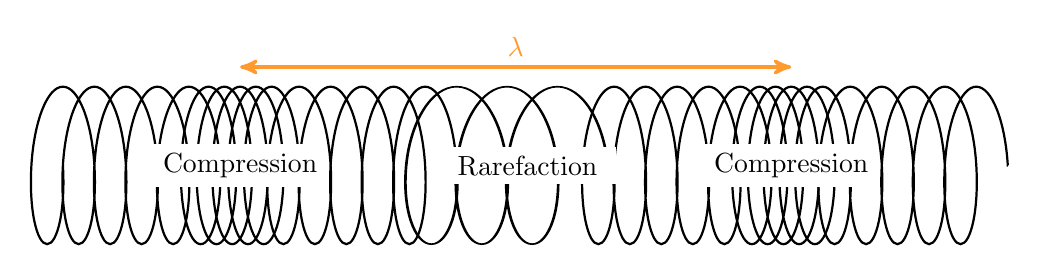
\begin{tikzpicture}[
	thick, decoration={coil, aspect=0.3, amplitude=-10mm},
	wave/.style={
		decorate, decoration={segment length=4mm}
	},
	compr/.style={
		decorate, decoration={segment length=2mm}
	},
	rare/.style={
		decorate, decoration={segment length=8mm}
	},
]

	\draw[wave]  (0cm, 0) -- (2cm, 0);
	\draw[compr] (2cm, 0) -- (3cm, 0);
	\draw[wave]  (3cm, 0) -- (5cm, 0);
	\draw[wave, transform canvas={xscale=1.6}, semithick]  (3.125cm, 0) -- (4.375cm, 0);
	%\draw[rare]  (5cm, 0) -- (7.41cm, 0);
	\draw[wave]  (7cm, 0) -- (9cm, 0);
	\draw[compr] (9cm, 0) -- (10cm, 0);
	\draw[wave]  (10cm, 0) -- (12cm, 0);
	
	\node [fill=white] at (2.25cm, 0) { Compression };
	\node [fill=white] at (5.9cm, 0) { \ Rarefaction \ };
	\node [fill=white] at (9.25cm, 0) { Compression };
	
	\draw [pfeil, <->] (2.25, 1.25) to node [color=MyColor2, sloped, above] {$\lambda$} (9.25, 1.25);
\end{tikzpicture}
	\caption{
		Illustration of a \textbf{longitudinal wave} exhibiting compression and rarefaction.
	}
	\label{fig:cmvis:longitudinal-wave}
\end{figure}

The ultrasound image formation process starts with the transducer sending out a short ultrasound pulse sequence into the body.
This pulse propagates as longitudinal wave (cf. Figure \ref{fig:cmvis:longitudinal-wave}) through the tissues and gets partly absorbed and reflected at different depths until these echoes eventually reach the transducer again where they are recorded.
After several processing steps and assuming a constant speed of sound of $1540 \frac{\text{m}}{\text{s}}$, the intensity and runtime of the ultrasound echoes, representing reflectance and depth, can be used to form a 2D image of the underlying anatomy.

\begin{figure}[ht]
	\centering
	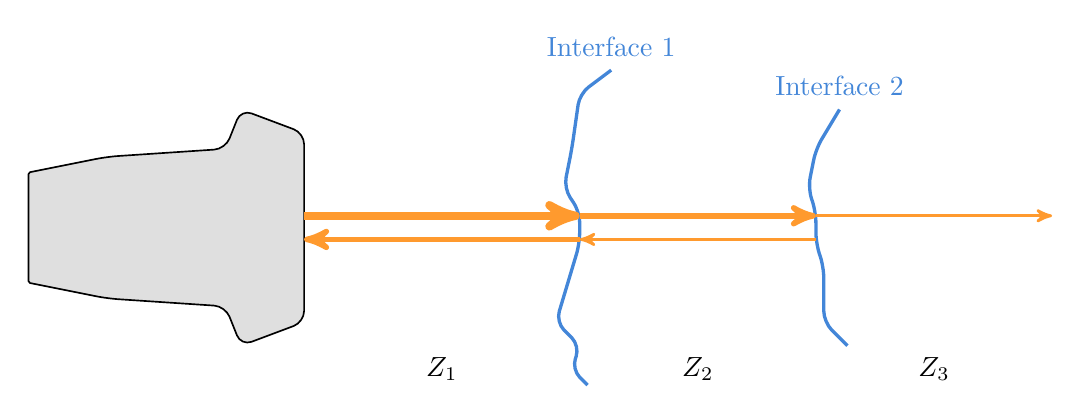
\begin{tikzpicture}[line join=round]
	% the transducer	
	\filldraw [color=black, fill=gray!25, semithick]
		(-10mm, 0cm) 
			to[rounded corners=0.2mm] (-10mm, 7mm) 
			to[rounded corners] (0mm, 9mm) 
			to[rounded corners] (15mm, 10mm) 
			to[rounded corners] (17mm, 15mm) 
			to[rounded corners] (25mm, 12mm) 
		-- (25mm, 0mm) 
			to[rounded corners] (25mm, -12mm) 
			to[rounded corners] (17mm, -15mm) 
			to[rounded corners] (15mm, -10mm) 
			to[rounded corners] (0mm, -9mm) 
			to[rounded corners=0.2mm] (-10mm, -7mm) 
		-- (-10mm, 0mm)
		;
	
	% Interface 1
	\draw [color=MyColor1, very thick, rounded corners, xshift=2cm]
		(44mm, 20mm) to (40mm, 17mm) to (39mm, 10mm) to (38mm, 5mm) to (40mm, 2mm) -- (40mm, -2mm) to (37mm, -12mm) to (40mm, -15mm) to (39mm, -18mm) to (41mm, -20mm);
	
	% Interface 2
	\draw [color=MyColor1, very thick, rounded corners, xshift=5cm]
		(43mm, 15mm) to (40mm, 10mm) to (39mm, 5mm) to (40mm, 2mm) -- (40mm, -2mm) to (41mm, -5mm) to (41mm, -12mm) to (44mm, -15mm);
	
	\node [color=MyColor1] at (64mm, 23mm) {Interface 1};
	\node [color=MyColor1] at (93mm, 18mm) {Interface 2};

	\node [color=black] at (42.5mm, -18mm) {$Z_1$};
	\node [color=black] at (75mm, -18mm) {$Z_2$};
	\node [color=black] at (105mm, -18mm) {$Z_3$};
	
	\draw [pfeil, line width=3pt] (25mm, 1.5mm) -- (60mm, 1.5mm);
	\draw [pfeil, line width=2pt] (60mm, -1.5mm) to (25mm, -1.5mm);
%	\draw [pfeil, line width=2pt] (60mm, -1.5mm) to node [sloped, below, color=MyColor2] {$R_1$} (25mm, -1.5mm);
	
	\draw [pfeil, line width=2pt] (60mm, 1.5mm) to (90mm, 1.5mm);
	\draw [pfeil, line width=1pt] (90mm, -1.5mm) to (60mm, -1.5mm);
	
	\draw [pfeil, line width=1pt] (90mm, 1.5mm) to (120mm, 1.5mm);
\end{tikzpicture}
	\caption{
		Simplified illustration of \textbf{reflection and transmission at tissue interfaces}.
		When an ultrasound wave crosses an interface between two tissues of different acoustic impedance, parts of the signal gets reflected while the remainder continues traveling through the anatomy (cf. Equation \ref{eq:cudacm:reflection-transmission-coefficients}).
	}
	\label{fig:cmvis:transducer-reflection}
\end{figure}

More precisely, the longitudinal ultrasound wave propagates areas of compression and rarefaction (cf. Figure \ref{fig:cmvis:longitudinal-wave}) through the anatomy inducing several different interactions with the tissue.
Within homogeneous media, the main \SYN{effect} is absorption where energy is dissipated over depth leading to a \SYN{mostly uniform} attenuation of the signal.
Furthermore, wave interference and diffraction, as well as further non-linear effects occur.
For diagnostic imaging however, the wave interactions with inhomogeneous media, namely reflection, transmission, refraction and scattering, are much more important.
Interfaces between two tissues of different acoustic impedance lead to a reflection of parts of the signal, while the remainder of the signal is further transmitted (cf. Figure \ref{fig:cmvis:transducer-reflection}), yielding a reflection coefficient $R_i$ and a transmission coefficient $T_i$:
\begin{equation}
	\label{eq:cudacm:reflection-transmission-coefficients}
	R_i	= \left( \frac{Z_2 - Z_1}{T_2 + Z_1} \right)^2, \quad
	T_i	= \frac{4Z_1 Z_2}{\left( Z_2 + Z_1 \right)^2}.
\end{equation}
According to Snell's law and the Fresnel equations, this reflection and transmission is angle dependent so that refraction \SYN{happens} and the direction of the longitudinal wave changes if an interface is not perpendicular to the wave front.
Since a tissue is never completely homogeneous, this process happens continuously and yields the characteristic ultrasound speckle patterns where the inhomogeneities are smaller than the wave length $\lambda$, often modeled as random point scattering.

This image formation process give B-mode ultrasound it's characteristic gradient-like appearance where the intensities rather show the changes in physical properties than the physical properties themselves.
In addition, these intensities are highly direction-dependent since the amount of observed reflection intensity decreases with increasing angle between sound direction and interface normal.
Thus, estimating signal attenuation and general uncertainty from B-mode image is a non-trivial task, for which different approaches have been presented \cite{Noble:2010:Ultrasound, Noble:2011:Ultrasound}.


\section{Confidence Maps for B-mode Ultrasound}
\label{sec:cudacm:cm}
%Introduce the concept of US Confidence Maps, and related work.

\begin{figure}[ht]
	\centering
	\subfloat[~Original liver ultrasound image.]{
		\label{fig:cudacm:liver_us}
		\includegraphics[width=0.47\linewidth]{figures/cudacm/liver_us.png}
	}
	\
	\subfloat[~Corresponding confidence map.]{
		\label{fig:cudacm:liver_cm}
		\includegraphics[width=0.47\linewidth]{figures/cudacm/liver_cm.png}
	}
	\caption{\textbf{Confidence maps on liver ultrasound}: (a) shows the original ultrasound image, (b) shows the corresponding confidence map, bright regions depicting regions of high confidence, dark regions depicting regions of low confidence.}
	\label{fig:cudacm:liver_us_cm}
\end{figure}

A \SYN{major} generalization of different concepts of ultrasound uncertainty estimation are ultrasound Confidence Maps, originally proposed by Karamalis et al. \cite{Karamalis:2012:ConfidenceMaps} and later refined by Hennersperger et al. \cite{Hennersperger:2014:EnergyMinimizationFramework}.
They describe a per-pixel estimation of the amount of uncertainty present in ultrasound images due to signal attenuation and shadowing, for which they employ a random walks formulation similar to the one by Grady to solve the $k$-label image segmentation problem \cite{Grady:2006:RandomWalks}.
Taking ultrasound physics into account, Confidence Maps describe the probability of a random walker starting from a given pixel to reach the virtual transducer elements.

\begin{figure}[ht]
	\centering
	\includegraphics[width=0.5\linewidth]{./figures/cudacm/diffusion_problem_8n.pdf}
	\caption{Illustration of the \textbf{diffusion graph network for computing Confidence Maps}. Each node is connected to its 8 neighborhood where the edge weights are defined as a function of the edge direction and gradients in the B-mode image.}
	\label{fig:cudacm:diffusion-graph}
\end{figure}

As illustrated in Figure \ref{fig:cudacm:diffusion-graph}, the image is represented as an undirected graph $G = (V, E)$, where the nodes $v \in V$ represent the image pixels, each being connected to its 8 surrounding nodes through the edges $e \in E$.
Each edge $e_{ij} \in E$, connecting nodes $v_i$ and $v_j$ is assigned a weight $w_{ij} > 0$ describing the likelihood of the random walker crossing that edge.
Furthermore, a set of virtual transducer elements are placed at the start and end of each ultrasound scanline to define the signal attenuation boundary conditions.
The edge weights are given as
\begin{equation}
	\begin{split}
		w_{ij} &= 
			\begin{cases}
				\exp(-\beta (|c_i - c_j| + \gamma))         & \text{if $i, j$ adjacent and $e_{ij}$ horizontal edge} \\
				\exp(-\beta (|c_i - c_j|))                  & \text{if $i, j$ adjacent and $e_{ij}$ vertical edge}   \\
				\exp \left(-\beta (|c_i - c_j| + \sqrt 2 \gamma) \right) & \text{if $i, j$ adjacent and $e_{ij}$ diagonal edge}   \\
				0                                           & \text{otherwise},
			\end{cases} \\
		c_i &= g_i \exp(-\alpha l_i),
	\end{split}
\end{equation}
where $g_i$ is the image intensity at node $i$ and $l_i$ describes the normalized closest distance to the virtual transducer elements.
The three free parameters $\alpha, \beta$ and $\gamma$ define the \SYN{outcome} of the Confidence Maps.
While the $\alpha$ parameter describes the likelihood of random walks along vertical edges and thus scales the estimated  attenuation with increasing depth, $\beta$ affects the robustness and accuracy of the segmentation result.
Furthermore, $\gamma$ penalizes random walks along the horizontal and diagonal edges and thereby \SYN{adjusts} the amount of horizontal discontinuities.
A more thorough discussion of the edge weights and the free parameters can be found in the original paper \cite{Karamalis:2012:ConfidenceMaps}.
In their evaluation, Karamalis et al. demonstrate that ultrasound Confidenece Maps describe an accurate per-pixel estimate of the signal attenuation, which can be translated to the amount of uncertainty present in the image.
Typical applications are ultrasound shadow detection, 3D freehand ultrasound compounding and multi-modal registration.

Due to the formulation as diffusion problem with Dirichlet boundary conditions, where the scanline sources have full confidence and the scanline sinks have zero confidence, Confidence Maps always exhibit the whole value range of $[0, 1]$.
Thus, the computed values describe only relative information with respect to the current image.
As a consequence, one has to pay special attention when comparing Confidence Maps of different images.
While the values of images of the same sequence may be comparable, confidence values between images of different anatomies are not directly numerically comparable.


\section{Traditional Implementations}
%Short discussion on traditional implementations using direct solves, such as LU decomposition.

Due to the formulation as Dirichlet diffusion problem, the computation of ultrasound Confidence Maps can be efficiently encoded in a linear system of the form
\begin{equation}
	L \mathbf{x} = \mathbf{b},
	\label{eq:cudacm:cm-system}
\end{equation}
where $L$ describes the Laplacian matrix of the graph, $\mathbf{x}$ is the Confidence Map in vectorized form and $\mathbf{b}$ encodes the Dirichlet boundary conditions.
Since, the graph is undirected and describes an 8-neighborhood, $L$ is symmetric, sparse, and positive definite.
Thus, Equation \ref{eq:cudacm:cm-system} is traditionally be solved with direct methods such as LU decomposition \cite{Karamalis:2012:ConfidenceMaps}.

Unfortunately, direct solvers do not \SYN{suit well} the interactive \SYN{characteristic} of ultrasound imaging.
Even with the relatively moderate resolution of ultrasound images, real-time computation of Confidence Maps is not feasible with today's hardware.
Karamalis et al. report computation times of \SYN{a little more} than two seconds \cite{Karamalis:2012:ConfidenceMaps}, which was reproduced by our experiments.
Chatelain et al. use Confidence Maps for servoing of robotic ultrasound \cite{Chatelain:2015:UltrasoundServoing}.
However, in order to yield interactive frame rates they had to significantly downsample the ultrasound images and it is unclear how much this \SYN{impairs} the quality of the results.
Thus, other methods are needed in order to solve Equation \ref{eq:cudacm:cm-system} in real-time.


\section{Real-Time Incremental Solving}
In order to yield real-time Confidence Maps for our system, we leverage the dynamic nature of ultrasound acquisitions and the temporal coherency of its images based on the high acquisition rates of today's systems.
Consecutive images in ultrasound sequences usually differ very little and therefore the corresponding Confidence Maps will likely be very similar.
We exploit this fact by using an iterative Jacobi-preconditioned Conjugate Gradient solver instead of directly solving Equation \ref{eq:cudacm:cm-system} through matrix decompositions.
This allows us to execute an incremental computation scheme, where we directly use the resulting Confidence Maps as initialization for the subsequent frame (cf. Figure \ref{fig:cudacm:incremental-computation}). 
This greatly reduces the number of needed iterations per frame as we have a better convergence to the true solution in the limited time budget available per frame. 

\begin{figure}[ht]
	\centering
	\includegraphics[width=0.75\linewidth]{./figures/cudacm/incremental-computation.png}
	\caption{Illustration of our proposed \textbf{incremental computation scheme} for Confidence Maps. Due to the temporal coherency of ultrasound imaging, consecutive images and thus also their Confidence Maps are usually very similar. Therefore, we use the each computed Confidence Map as initialization for the iterative solving of the subsequent frame.}
	\label{fig:cudacm:incremental-computation}
\end{figure}

We construct the equation system matrix $L$ explicitly on each frame.
Due to the given graph \SYN{layout}, the matrix has only 9 diagonals with non-zero entries and can thus be efficiently stored using the sparse DIA matrix storage format \CN.
For the very first frame, we initialize $x$ with a linear gradient as very rough approximation of the Confidence Map.
Then, for every subsequent frame, we use the computed result as initialization.
For easier integration with visualization techniques and to allow for an interactive experience in general, we implemented our technique on the GPU using CUDA.
The preconditioned Conjugate Gradient solver has a specific time budget depending on the target frame rate, in which it performs as many iterations as possible.
Even though this time budget might be too small to yield exact solutions from the beginning, our later evaluation shows, that the temporal coherency of ultrasound sequences is sufficient to have the solver converge within very few frames.

\begin{figure}[t]
	\centering
	\begin{tikzpicture}[
	schritt/.style={
		schritt-base, rectangle split, rectangle split parts=2, minimum height=8mm, minimum width=28mm
	},
	entity/.style={
		entity-base, minimum height=8mm, minimum width=22mm
	},
	portL/.style={
		font=\sffamily\scriptsize, outer xsep=1mm,
		align=left, anchor=west,
	},
	portR/.style={
		font=\sffamily\scriptsize, outer xsep=1mm,
		align=right, anchor=east,
	},
	pfeilkurz/.style={
		pfeil, shorten >=0.5mm
	},
	node distance=6mm and 10mm
	]

	\node (filter) [schritt] { \phantom{p}\textbf{Image Filter}\phantom{b} \nodepart{two}\\ };	
	\PORT{2L1}{($ (filter.two west) + (0, 0mm) $)}{MyColor2}{node[portL] {Input \phantom{pb}}}
	\PORT{2R1}{($ (filter.two east) + (0, 0mm) $)}{MyColor2}{node[portR] {\phantom{pb} Resampled US}}
%	\PORT{2R2}{($ (filter.two east) - (0, 2mm) $)}{MyColor2}{node[portR] {\phantom{pb} Blurred US}}

	\node (igtlink) [entity, left=of filter] {\textbf{US Image}};
	\PORT{1R1}{($ (igtlink.east) - (0mm, 0mm) $)}{MyColor2}{}
	
	\node (cmsolver) [schritt, right=of filter] { \textbf{Confidence Map Solver} \nodepart{two}\\\\ };	
	\PORT{4L1}{($ (cmsolver.two west) + (0, 2mm) $)}{MyColor4}{node[portL] {Initial Solution \phantom{pb}}}
	\PORT{4L2}{($ (cmsolver.two west) - (0, 2mm) $)}{MyColor2}{node[portL] {US Image \phantom{pb}}}
	\PORT{4R1}{($ (cmsolver.two east) + (0, 2mm) $)}{MyColor4}{node[portR] {\phantom{pb} CM}}

%	\node (ucmapping) [schritt, right=of cmsolver]{ \textbf{Uncertainty Mapping} \nodepart{two}\\\\\\\\ };	
%	\PORT{5L1}{($ (ucmapping.two west) + (0, 4mm) $)}{MyColor4}{node[portL] {CM \phantom{pb}}}
%	\PORT{5L2}{($ (ucmapping.two west) - (0, 0mm) $)}{MyColor2}{node[portL] {Blurred Image \phantom{pb}}}
%	\PORT{5L3}{($ (ucmapping.two west) - (0, 4mm) $)}{MyColor2}{node[portL] {B-mode US \phantom{pb}}}
%	\PORT{5R1}{($ (ucmapping.two east) + (0, 4mm) $)}{MyColor2}{node[portR] {\phantom{pb} Fused US}}

	\node (scanline) [entity, right=of cmsolver] { \textbf{Confidence Map} };
	\PORT{6L1}{($ (4R1) + (10mm, 0mm) $)}{MyColor4}{}
	
	
	\begin{pgfonlayer}{background}
		\draw [pfeilkurz] (1R1) to [out=0, in=180, in distance=6mm] (2L1);
%		\draw [pfeilkurz] (1R1) |- ($ (5L3) - (4mm, 6mm) $) |- (5L3);
	
		\draw [pfeilkurz] (2R1) to [out=0, in=180, in distance=6mm] (4L2);
%		\draw [pfeilkurz] (2R2) -| ($ (2R2) + (4mm, -4mm) $) |- ($ (5L2) - (6mm, 8mm) $) |- (5L2);
	
		\draw [pfeilkurz, draw=MyColor4] (4R1) -| ($ (4R1) + (3mm, 4mm) $) |- ($ (4R1) + (0mm, 11mm) $) -| ($ (4L1) + (-5mm, 4mm) $) |- (4L1);
%		\draw [pfeilkurz, draw=MyColor4] (4R1) -- ($ (4R1) + (3mm, 0mm) $) to ($ (5L1) - (5mm, 0mm) $) -- (5L1);
	
		\draw [pfeilkurz, draw=MyColor4] (4R1) -- (6L1);
	\end{pgfonlayer}{background}

\end{tikzpicture}
	\caption{
		\TODO{Redo this illustration to show only the cudacm parts, not the cmvis parts.}
		\textbf{Processing pipeline} of our reference implementation. We receive the original ultrasound B-mode image through OpenIGTLink and perform an Gaussian blur and a resampling in order to improve the PCG convergence performance. 
		The Confidence Map solver then incrementally computes the B-mode image's Confidence Map by using the previous image's Confidence Map as initialization. 
		Finally, we perform the uncertainty mapping using one of the three presented schemes (cf. Section \ref{sec:cmvis:mapping-schemes}) and transform the image from polar to cartesian coordinates.
	}
	\label{fig:cmvis:campvis_pipeline}
\end{figure}

As already discussed in Section \ref{sec:cudacm:cm}, Confidence Maps exhibit only a relative measure of confidence.
Their strength is not the exact confidence value at a single pixel, but rather the distribution within the image.
Thus, due to noise in the original ultrasound, the Confidence Maps of multiple consecutive frames may exhibit a flickering behavior when being watched in a sequence.
To introduce a better temporal coherency, we apply an additional alpha beta filter \cite{Brookner:1998:Filtering}.
Being a variant of the Kalman filter, it recursively operates on the stream of computed Confidence Maps and produces a smoothened version by averaging the current image with a prediction based on the previous images.
We empirically selected a configuration of $\alpha = 0.36$ and $\beta = 0.005$ providing good results with both damping of flickering and preservation of the original confidence distribution and temporal responsiveness of the estimates.


\section{Evaluation}
\label{sec:cudacm:evaluation-performance}
For the evaluation of our methods, we had a professional sonographer acquire several sequences of patient abdominal ultrasound.
Our system was run on a Linux notebook with an Intel i7 processor and a nVidia GTX 750M GPU. 
Instead of acquiring live images from the ultrasound machine, we streamed the pre-recorded sequences from the hard disk via OpenIGTLink link, each containing 392 images of 512x512 pixels resolution.
To examine the influence of the system performance with respect to the different parameters, we ran our real-time solver in various configurations.

\paragraph{Resample Scale vs. Number of Iterations}
The analytical solving of Equation \ref{eq:cudacm:cm-system} using standard Cholesky decomposition requires an average of more than 2.2 seconds per frame and is thus far from real-time.
In contrast, our proposed incremental solver scheme allows to stop the iteration process at any time and use the best possible solution that can be computed within a give time budget.
We set this to $30$ms in order to ensure real-time applications with a target frame of $30$ fps.
\begin{figure}[ht]
	\centering
	\includegraphics[width=0.75\textwidth]{{figures/cudacm/evaluation/runtime_30ms}.png}
	\caption{
		\textbf{Solver runtime per frame} for the kidney data set with different configurations of PCG iterations and resample scales targeting $30$ms per frame.
		Smaller images yield a smaller problem size and thus allow for a higher number of iterations.
	}
	\label{fig:cudacm:evaluation-30ms}
\end{figure}
As shown in Figure \ref{fig:cudacm:evaluation-30ms}, the image size has a significant impact on the runtime performance, since the problem size can be significantly reduced by resampling the ultrasound images to a smaller resolution, compute the corresponding Confidence Maps and then upsample the result to back the original resolution.
While our test platform allows for only $30$ PCG iterations in full resolution, $50$ iterations are feasible with a resample scale of $0.75$ in each direction and over $100$ iterations are possible with a resample scale of $0.5$ in each direction.
Though the frame rates are rather constant, a jitter in the computation times is present.
Therefore, we do not limit our incremental solver by the number of iterations but by a given time budget.


\paragraph{Resample Scale vs. Image Quality}
While it is no surprise that smaller images allow for a higher number of PCG iterations, the interesting question is what impact the downsampling has on the image quality of the computed Confidence Maps.
We use the Structured Similarity Index Measure (SSIM) with a window size of $9 \times 9$ pixels \cite{Wang:2004:SSIM} for a quantitative comparison of our results with the exact reference solution.
This \SYN{makes sense} since we intend to use our real-time uncertainty estimation framework mainly for visualization purposes.
By modeling perceptual effects through \SYN{comparing} the covariance between the two images with their individual variances, the SSIM provides an excellent quantitative assessment of the perceived image quality.

\begin{figure}[ht]
	\centering
	\subfloat[~Minimal SSIM per frame for kidney data set.]{
		\includegraphics[width=0.49\textwidth]{figures/cudacm/evaluation/kidney_minssim_30ms.png}
	}
	\subfloat[~Minimal SSIM per frame for gullbladder data set.]{
		\includegraphics[width=0.49\textwidth]{figures/cudacm/evaluation/gullbladder_minssim_30ms.png}
	}
	\caption{
		Evaluation on the \textbf{image quality with respect to the resample scale} in terms of structural similarity.
		When maintaining a target time budget of 30ms, a lower resample scale yields a better image quality.
	}
	\label{fig:cudacm:evaluation-30ms-error}
\end{figure}

Smaller images exhibit both a smaller computational burden and a higher convergence rate of the solver, so that the resampling may even be beneficial for the resulting image quality.
However, at the same time, the lower resolution of the images may remove little details, which are important for the correct estimation of the signal attenuation.
When looking at Figure \ref{fig:cudacm:evaluation-30ms-error}, one can see that in general a slight downsampling of the images is benefitial for the final image quality.
For a couple of frames however, in particular with the kidney data set, details get lost yielding a worse structural similarity applying less PCG iterations on the full scale images.
With these results, we decided that using a resample scale of $0.5$ defines a good trade-off between computation time and image quality (cf. Figure \ref{fig:cudacm:evaluation-30ms-error}).


\paragraph{PCG Iterations vs. Image Quality}
As a final quantitative evaluation, we ran our proposed solver scheme with a fixed resample scale of $0.5$ but different number of iterations.
As illustrated in Figure \ref{fig:cudacm:performance_evaluation}, the SSIM never falls below $0.94$ when performing $110$ PCG iterations, which is an excellent result.
\begin{figure}[ht]
	\centering
	\subfloat[~Minimal SSIM per frame for kidney data set.]{
		\includegraphics[width=0.49\textwidth]{{figures/cudacm/evaluation/kidney_iterations_vs_minssim_0.50}.png}
	}
	\subfloat[~Minimal SSIM per frame for gullbladder data set.]{
		\includegraphics[width=0.49\textwidth]{{figures/cudacm/evaluation/gullbladder_iterations_vs_minssim_0.50}.png}
	}
	\caption{
		\textbf{Error (residual norm) over time} for different PCG iteration counts. 
		The resample scale was fixed to 0.5.
	}
	\label{fig:cudacm:performance_evaluation}
\end{figure}
For comparison, the dashed lines show the error progression when the solver is reinitialized at each iteration, which yields mostly worse results than 20 incremental iterations.
This demonstrates the importance of leveraging the dynamic nature of ultrasound and the effectiveness of our technique using the solution of the previous frame as initialization.
Table \ref{tbl:cudacm:kidney-results} further summarizes the results and shows the average runtime, average SSIM and minimum SSIM over the entire kidney data set.
One can see that the $110$ incremental PCG iterations of our reference implementation are real-time capable and yielding almost exact results with an average SSIM of $0.999$ and a minimum SSIM of only $0.941$.
Figure \ref{fig:cudacm:kidney-qualitative} presents qualitative results on a representative frame of the same ultrasound sequence.

\begin{table}[ht]
	\centering
	\begin{tabu} to 0.9\linewidth {>{\bfseries\centering}m{35mm} C C C}
		\toprule
		\multirow{2}{*}{\# Iterations} & \ \bfseries Avg. Runtime \ & \bfseries Avg. Quality & \bfseries Min. Quality    \\
		                               & \ \emph{(ms)} \            & \multicolumn{2}{c}{\emph{(Structural Similarity)}} \\
		\midrule
		Direct solver                  & \ $2214.68$ \              & \ $1.0$ \              & \ $1.0$ \                 \\
		\midrule
		20 (incremental) \             & \ $10.84$ \                & \ $0.991$ \            & \ $0.837$ \               \\
		50 (incremental) \             & \ $18.07$ \                & \ $0.997$ \            & \ $0.899$ \               \\
		80 (incremental) \             & \ $25.37$ \                & \ $0.998$ \            & \ $0.929$ \               \\
		110 (incremental) \            & \ $32.46$ \                & \ $0.999$ \            & \ $0.941$ \               \\
		\midrule
		110 (discarding) \             & \ $32.59$ \                & \ $0.984$ \            & \ $0.856$ \               \\
		\bottomrule
	\end{tabu}
	\caption{
		Aggregated \textbf{performance results in terms of runtime an error} with different configurations for the number of iterations. 
		The resample scale was fixed to 0.5. 
		Data set was a patient kidney ultrasound sequence containing a total of 392 frames.
	}
	\label{tbl:cudacm:kidney-results}
\end{table}

\begin{figure}[p]
	\centering
	\subfloat[~Original ultrasound frame from kidney sequence.]{
		\includegraphics[width=0.46\textwidth]{figures/cudacm/evaluation/cm_stuff/329_us.png}
	}
	\quad
	\subfloat[~Corresponding Confidence Map.]{
		\includegraphics[width=0.46\textwidth]{figures/cudacm/evaluation/cm_stuff/329_512_5000_cm.png}
	} 
	\\
	\subfloat[~Computed Confidence Map with 30 iterations in full resolution ($30$ms).]{
		\includegraphics[width=0.46\textwidth]{figures/cudacm/evaluation/cm_stuff/329_512_30_cm.png}
	}
	\quad
	\subfloat[~Structured Similarity between (b) and (c); average: $0.984$, minimum: $0.889$.]{
		\includegraphics[width=0.46\textwidth]{figures/cudacm/evaluation/cm_stuff/329_512_30_ssim.png}
	}
	\\
	\subfloat[~Computed Confidence Map with 100 iterations in half resolution ($30$ms).]{
		\includegraphics[width=0.46\textwidth]{figures/cudacm/evaluation/cm_stuff/329_256_110_cm.png}
	}
	\quad
	\subfloat[~Structured Similarity between (b) and (e); average: $0.998$, minimum: $0.973$.]{
		\includegraphics[width=0.46\textwidth]{figures/cudacm/evaluation/cm_stuff/329_256_110_ssim.png}
	} \\
	\caption{
		\textbf{Qualitative results of the presented incremental solver scheme}.
		By comparing (b) with (c) and (e), one can see the impact of the limited amount of iterations on the resulting Confidence Maps.
		The SSIM in (d) and (f) quantifies the perceptual difference.
		For better visualization of differences, the color map in (d) and (f) was normalized to the range of $[0.85, 1.0]$ and does not show the full SSIM range of $[-1, 1]$.
	}
	\label{fig:cudacm:kidney-qualitative}
\end{figure}


\section{Conclusion}
%\TODO{Write a conclusion for this chapter}
We presented a method to bring the estimation of B-mode ultrasound signal attenuation into real-time applications.
Building on ultrasound Confidence Maps, originally proposed by Karamalis et al. \cite{Karamalis:2012:ConfidenceMaps}, we propose an incremental solver scheme, which leverages the temporal coherency of ultrasound imaging.
In an extensive evaluation with clinical patient data, we assessed the impact of our different optimizations on the quality of the computed Confidence Maps and showed that our methods yield accurate approximations within a $30$ms time budget.
In the remainder of this thesis, we will use this work to generate real-time uncertainty informations for different ultrasound processing and visualization techniques.

%% !TEX root = ../thesis-example.tex
%
\chapter{Uncertainty Visualization for 2D Ultrasound}
\label{chap:cmvis}

Though there are many advantages of ultrasound imaging, such as being rather low-cost and real-time capable, the correct interpretation of B-mode images is a non-trivial task that requires a large amount of experience and training.
Even ultrasound experts sometimes struggle in performing an ultrasound-based diagnosis due to the presence of many different kinds of artifacts and it's non-homogeneous distribution of uncertainty.
In this chapter we present novel visualization techniques that augment the B-mode images with uncertainty information in real-time in order to support both ultrasound novices and expert users in gaining a better understanding of ultrasound.
Therefore, we build upon the previously introduced method of real-time confidence estimation for B-mode ultrasound images (cf. Chapter \ref{chap:cudacm}) and interpret these Confidence Maps as per-pixel uncertainty information, which we expose to the user using perceptual visualization techniques.
After a review on general uncertainty visualization techniques for medical applications, we discuss the clinical significance of our proposed system.
In total, we present three different visualization schemes for both educational and clinical applications and motivate the selection of visual variables to depict uncertainty in B-mode ultrasound images.
An extensive evaluation conducted with both ultrasound novices and expert clinicians demonstrates the usefulness of our techniques.
Parts of this work have been published in \CN.


\section{Uncertainty in Health Care and Medical Visualization}
\label{sec:cmvis:uncertainty-vis-techniques}
When \SYN{having} a comprehensive look at health care, the concept of uncertainty is ubiquitous throughout all levels.
However, since clinicians have been trained to make decisions and provide their patients with answers, many of them struggle to admit that their work is based on a plethora of input factors, each inducing an individual level of uncertainty, and thus their eventual findings rather represent the most likely interpretation than the \SYN{absolute truth}.

Han et al. investigate the different concepts and appearances of uncertainty in general health care using cancer treatment as example and derive a conceptual taxonomy in \cite{Han:2011:UncertaintyInHealthCare}.
They point out that a coherent concept of uncertainty in health care is missing and that multiple meanings and interpretations of that term are present, which are not necessarily distinguished from each other.
They conclude that uncertainty is actually a threefold concept which can originate either through probability, ambiguity or complexity with issues ranging from disease-centered to patient-centered ones.

While the paper of Han et al. analyzes the problem from the clinical perspective, Ristovski et al. focus on the various technical aspects and investigate the presence of uncertainty in medical visualization \cite{Ristovski:2014:UncertaintyInMedVis}.
As introduced in Section \ref{sec:background:vis:vispipeline}, the visualization pipeline ranges from the initial acquisition of data, over several data processing steps to the final rendering output.
Though each of these steps is subject to an individual level of uncertainty, the final rendering often shows the data as if it were the only possible truth.
However, it requires appropriate visualization to make the amount of uncertainty assessable to the clinician and thereby propagate the information back correctly to the clinical perspective as it was previously presented by Han et al.
For instance, Lundström et al. point out that a suboptimal setup of a transfer function during rendering can lead to a false classification of stenosis \cite{Lundstrom:2007:Animation}.

\begin{figure}[ht]
	\centering
	\includegraphics[width=0.75\linewidth]{figures/cmvis/rieder-rfablation.jpg}
	\caption{
		Uncertainty visualization of radio-frequency ablation zones as proposed by Rieder et al. \cite{Rieder:2011:AblationApproximation}.
	}
	\label{fig:cmvis:rieder-rfablation}
\end{figure}

The special setup in which medical visualization is used and its resulting requirements make it difficult to apply techniques from other domains, such as \cite{Pfaffelmoser:2011:VisualizingVariability, Pothkow:2011:PositionalUncertainty}, even though they use very similar data.
This may be one of the reasons why the body of literature on medical uncertainty visualization is rather shallow and the individual works are very application- and task-specific.
One such example is the uncertainty visualization technique of Rieder et al. proposed in the context of percutaneous radio-frequency ablation.
For this application, precise planning of the applicator placement is crucial in order to ensure that the malignant tissue is destroyed completely (cf. Figure \ref{fig:cmvis:rieder-rfablation}).
Their work is particularly noteworthy as they use their visualization for the optimization of a seven-dimensional optimization problem (five degrees of freedom for the placement of each needle plus two free simulation parameters) in three-dimensional space \cite{Rieder:2011:AblationApproximation}.
Another similar approach is the work of Brecheisen et al. exploring the parameter sensitivity in fiber tracking algorithms for DTI data \cite{Brecheisen:2009:ParameterSensitivy}.
Both techniques rely on interactive exploration by the user in order to cover the available parameter space.

\begin{figure}[ht]
	\centering
	\includegraphics[height=4cm]{figures/cmvis/prassni-uncertainty1.jpg}
	\qquad
	\includegraphics[height=4cm]{figures/cmvis/prassni-uncertainty2.jpg}
	\caption{
		Uncertainty visualization of segmentation algorithm results as proposed by Prassni et al. \cite{Prassni:2010:Uncertainty}.
	}
	\label{fig:cmvis:prassni-uncertainty}
\end{figure}

One example of providing feedback on the uncertainty present in medical imaging algorithms is the work of Praßni et al.
They propose a guided probabilistic volume segmentation technique for which they visualize the resulting uncertainty distribution using iso-lines and opacity modulation (cf. Figure \ref{fig:cmvis:prassni-uncertainty}).
As mentioned previously, it is crucial to expose information on the result quality to the clinician, since ultimately they have to decide on diagnosis and treatment.
The recent progress on ensemble visualizations \cite{Hao:2016:TemporalEnsembles, Obermaier:2014:FutureEnsemble, Rautenhaus:2015:EnsembleVisualization} could be influential for further progress in this direction.
In the medical domain such techniques can for instance be used to visualize the results of large random studies on medical imaging algorithms and thereby make them more accessible.




\section{Clinical Significance and Application}
\label{sec:cmvis:clinical-significance}

Compared to other anatomical medical imaging modalities such as CT or MRI, medical ultrasound exhibits several benefits, such as being comparatively cheap, portable and real-time capable.
It is therefore widely used in today's clinical practice, for instance for abdominal, pediatric, head and general vascular applications \cite{Noble:2011:Ultrasound}. 
However, acquiring a good image (e.g. in terms of high diagnostic value) is a non-trivial task due to the highly complex ultrasound image formation process (cf. Section \ref{sec:cudacm:us-image-formation}).
It is influenced by various physical imaging parameters such as frequency, focus, and depth, as well as by external factors such as probe positioning, probe pressure, patient positioning and patient breathing cycle \cite{Aldrich:2007:USPhysics}, and can yield a wide range of image artifacts \cite{Scanlan:1991:Artifacts}.
Furthermore, some target anatomies can not be directly reached but need to be scanned by circumventing strong reflectors such as bones, which prevent the acquisition of images underneath.
A classic example of such an anatomy are the kidneys, which can not be scanned from the back as they are then in the acoustic shadow of the spine reflecting almost all ultrasound waves.
Instead, sonographers perform kidney ultrasound through the abdomen, usually using the liver as an acoustic window since it has the best transmission properties of the surrounding anatomy.

\begin{figure}[ht]
	\centering
	\subfloat[]{
		\includegraphics[width=0.42\linewidth]{figures/cmvis/liver_high_uncertainty.jpg}
	}	
	\qquad
	\subfloat[]{
		\includegraphics[width=0.42\linewidth]{figures/cmvis/liver_low_uncertainty.jpg}
	}
	\caption{
		\textbf{Kidney ultrasound using the liver as acoustic window} with applied uncertainty visualization using chroma as visual variables (cf. Section \ref{sec:cmvis:mapping-schemes}).
		A slight repositioning of the transducer results in a considerable increase of confidence in image (b) compared to (a).}
	\label{fig:cmvis:kidney_acoustic_window}
\end{figure}

Sonographers need to be aware of all these caveats of ultrasound imaging in order to correctly understand the image.
In particular medical trainees and ultrasound novices have difficulties in getting the right image needed for their clinical objectives since traditional ultrasound imaging does not provide a direct qualitative feedback on the image quality.
Already a slight repositioning of the transducer can yield a significantly better acoustic window and thus improve the image for the target anatomy (cf. Figure \ref{fig:cmvis:kidney_acoustic_window}).
Thus, training is an important aspect for medical students when learning ultrasound \cite{Butter:2007:UsTraining}.
In particular in trauma applications, where time is critical, the surgeon has to determine possible fractures and lesions as quickly as possible and has a minimal margin for error \cite{Knudtson:2004:TraumaSuite}.
With this motivation in mind, we developed our work with the aim to support both medical students in learning sonography as well as expert clinicians for a more quick and intuitive interpretation of ultrasound images by providing an interactive feedback on the image quality and uncertainty distribution.


\section{Selection of Visual Variables}
\label{sec:cmvis:selection-visual-variables}

Essentially, we target two different applications with our work:
On the one hand, we are convinced that exposing uncertainty information to ultrasound novices and trainees helps them to better understand the complex ultrasound image formation process.
At the same time, we also expect expert sonographers to benefit from uncertainty visualization as the additional information may improve the diagnostic value of the image.
Regarding these two target applications, we yield the following requirements for ultrasound uncertainty visualization schemes.
\begin{my_list_item}
	\item 
		The uncertainty information should be fused directly into the original B-mode sequence. Thus, both the spatial and the temporal domain are fixed.
		
	\item
		The primary information in the uncertainty maps are not the exact per-pixel uncertainty values but the distribution of the uncertainty with respect to the anatomy (cf. Section \ref{sec:cudacm:cm}).
		
	\item
		For educational applications, the uncertainty distribution in the image should be easily and intuitively perceivable. Even small changes in the uncertainty distribution should be clearly observable when repositioning the ultrasound probe in order to maximize the learning effect.
		
	\item
		For clinical applications, the diagnostic information in the B-mode image must not be impaired. Thus, the original image intensities should be preserved as good as possible and no image regions should be occluded.
\end{my_list_item}
Given these requirements for our uncertainty visualization, the number of viable visual variables for depicting the uncertainty information is limited.

One traditional technique is the usage of glyphs for depicting uncertainty, with error bars in 1D visualization being the classic example.
Glyphs have the advantage of offering a large number of visual variables that can be used to alter their appearance.
For instance, MacEachren et al. evaluate 11 different mappings of uncertainty to point glyphs \cite{MacEachren:2012:VisualSemiotics}.
Glyphs excel in depicting uncertainty when used in sparse layouts allowing the observer to individually focus on single glyphs in order to read their information.
However, this does not work well for our application where the goal is to visualize the distribution of a dense 2D scalar field.
Although dense glyph fields have also been successfully used for depicting global information \cite{Kindlman:2006:GlyphPacking, Borgo:2012:GlyphVisualization}, we do not consider them for our work since early experiments did not show promising results.
The work of Sanyal et al. supports this fact as their experiments showed that in many uncertainty related tasks on 2D data sets the different glyph mappings perform significantly worse than surface color mapping \cite{Sanyal:2009:UncertaintyVis}.
Furthermore, adding glyphs to the B-mode image would occlude the original ultrasound image, which is undesirable for clinical applications.

One intriguing approach is to extend the 2D data to the third dimension and map uncertainty to the Z axis in a 3D rendering \cite{Brown:2004:VibrationVis, Kao:2001:Eosvis}.
While this may be a valid method for applications such as geospatial visualization, it can not be applied to our use case since, due to the 2D projection of a 3D scene, it requires the user to interact with the camera to get the full information.
Furthermore, as mentioned above, the spatial domain of our visualization is fixed as clinicians expect a 2D image when performing 2D B-mode ultrasound.

Another approach is to exploit the spatial domain for depicting uncertainty, for instance through animations, animated jittering or probabilistic animation \cite{Brown:2004:VibrationVis, Lundstrom:2007:Animation}.
However, since we are working with real-time ultrasound sequences, the temporal domain is fixed and such approaches are not applicable.
\TODO{extend the last two paragraphs/this section}


\section{Visualization Schemes}
\label{sec:cmvis:mapping-schemes}

Given these considerations and the particular requirements of our intended uncertainty visualization, we selected the visual variables of color and texture.
They both do not affect the spatial and temporal image domain and are very powerful and intuitive for expressing general uncertainty \cite{MacEachren:2012:VisualSemiotics}.
In total, we propose three different uncertainty mapping techniques for the two applications, which we will discuss in detail in the following sections.
Since both the B-mode image and the uncertainty map are in the same image domain, no coordinate transformation is necessary and the mapping techniques are focused on the optical properties.

\begin{figure}[ht]
	\centering
	\begin{tikzpicture}[%
	schritt/.style={%
		schritt-base, minimum height=8mm, minimum width=20mm%
	},%
	entity/.style={%
		entity-base, minimum height=8mm, minimum width=20mm%
	}, %
	box/.style={%
		rectangle, align=center, %
		thick, draw=black!42, %
		inner sep=0.2cm%
	}, %
	node distance=4mm and 8mm%
]%
	
	\node (pta) [font=\scriptsize, align=center] {Evaluate\\ on Each \\ Sample};
	\node (cm) [entity,right=of pta,yshift=0.6cm,xshift=-0.6cm] {Color\\ Modulation};
	\node (importances) [entity,below=of cm] {Importance};
	
	\node (ptabox) [box, schritt, fit={(pta) (cm) (importances)}] {};
	
	\node (pta2) [font=\scriptsize, align=center] {Evaluate\\ on Each \\ Sample\\ };
	\node (cm2) [entity,right=of pta,yshift=0.6cm,xshift=-0.6cm] {Color\\ Modulation};
	\node (importances2) [entity,below=of cm] {Importance};
	
	\node (sp) [entity,left=of ptabox,xshift=2mm] {Predicate Histogram};
	
	\node (select) [schritt,left=of sp,xshift=2mm] {Select, Combine \& \\ Configure Predicates };
	\node (lib) [entity,above=of select,yshift=0.2cm] {Point Predicate\\ Library};
	\node (wfm) [entity,below=of select,yshift=-0.2cm] {Workflow Model};

	\node (am) [entity,below=of ptabox,yshift=-0.1cm] {Anatomical Model};
	
	\node (classification) [schritt,right=of cm,xshift=2mm] {Classification};
	\node (sampling) [schritt,above=of classification] {Sampling};
	\node (usi) [entity,above=of sampling,xshift=-2cm] {Ultrasound Image};
	\node (compositing) [schritt,below=of classification] {Focus \& Context \\ Compositing};
	\node (result) [entity,below=of compositing,yshift=-0.2cm] {Rendered Image};
	
	\node (dvr) [font=\scriptsize, align=center, right=of classification, xshift=-0.6cm] 
		{~\\ Direct \\ Volume \\ Rendering \\ Pipeline};
	\node (dvrbox) [box, fit={(classification) (sampling) (compositing) (dvr)}] {};
	
	\path 
		(lib) edge[pfeil] (select)
		(wfm) edge[pfeil] (select)
		
		(select) edge[pfeil] (sp)
		(sp) edge[pfeil] (ptabox)
		(am) edge[pfeil] (ptabox)
		
% 			(usi) edge[pfeil] (sampling)
		(sampling) edge[pfeil] (classification)
		(classification) edge[pfeil] (compositing)
		(compositing) edge[pfeil] (result)

		(cm) edge[pfeil] (classification)
		(importances) edge[pfeil] (compositing);

	\draw[|-,pfeil] (usi.west) -| (ptabox.north);
	\draw[|-,pfeil] (usi.east) -| (sampling.north);
% 		\draw[|-,pfeil] (ptabox.east) |- (sampling.west);
\end{tikzpicture}
	\caption{
		\textbf{Schematic diagram} of the different proposed uncertainty visualization schemes.
		Given the original B-mode ultrasound image $I$, we compute its Confidence Map $CM$ and a Gaussian blurred version $G_\sigma$. 
		The uncertainty map $U$ is derived from $CM$ by inverse linear mapping (cf. Equation \ref{eq:cmvis:u-from-cm}). 
		For the color overlay and the uncertainty mapping to chroma, we compute a derived uncertainty measure $U'$ using a transfer function. 
		Finally, the uncertainty information is fused into the original ultrasound image using one of the three visualization schemes.
	}
	\label{fig:cmvis:schematic-diagram}
\end{figure}

As illustrated in Figure \ref{fig:cmvis:schematic-diagram}, all proposed mapping schemes start with the original B-mode ultrasound image $I$, for which we compute the corresponding Confidence Map.
We assume it to be inversely related to the amount of uncertainty in the image, more precisely to it's facets of accuracy, precision and credibility.
Thus, we obtain the per-pixel uncertainty information $U$ by applying a direct inverse linear mapping
\begin{equation}
	\label{eq:cmvis:u-from-cm}
	U(x) := 1 - CM(x),
\end{equation}
where $CM(x) \in [0,1]$ is the confidence map value at pixel $x$ in the image domain.


\subsection{Uncertainty as Color Overlay}
\label{sec:cmvis:color-overlay}
For educational applications, the focus of the visualization should be on the uncertainty information and even small changes in the distribution should be clearly distinguishable by the observer.
At the same time, the corresponding ultrasound B-mode image should be shown as anatomical reference in order to allow for an understanding of the connection between image features and their effects on the uncertainty.
Therefore, we combine the visual variables of hue and value in our proposed color overlay scheme (cf. Figure \ref{fig:cmvis:schematic-diagram}).
Compared to the other presented mapping schemes, the combination of the two visual variables makes even subtle changes of uncertainty visible to the observer.
We deem this an important feature to teach ultrasound novices the caveats of the ultrasound image formation process.


As previously introduced, for each pixel $x$, let $U(x)$ be its uncertainty value and $I(x)$ be its original B-mode intensity.
Since the color overlay is a very obtrusive mapping scheme, we use a transfer function to apply a thresholding to the uncertainty measure and define the derived uncertainty as $U'(x) := \max \left( 0, \, 2 U(x) - 1 \right)$.
Using this derived measure instead of the original $U(x)$ avoids overlaying regions of negligible uncertainty.
We first generate the color overlay in HSV color space as
\begin{equation}
	C(x)_{HSV} := \left( H, U'(x), V \right),
\end{equation}
with constant hue $H \in [0, 1]$ and constant value $V \in [0, 1]$.
We chose a bright orange color with $H = 0.15$ and $V = 0.8$ to avoid lowering the contrast to Doppler ultrasound utilizing the colors blue and red.
In a second step, we linearly mix the color overlay transformed to RGB color space with the original B-mode to yield the final pixel color 
\begin{equation}
	O(x) := U'(x) \cdot C_{RGB}(x) + \left( 1 - U'(x) \right) \cdot I(x).
\end{equation}
Figure \ref{fig:cmvis:vis-color-overlay} shows the uncertainty color overlay applied to two different abdominal ultrasound images.

\begin{figure}[ht]
	\centering
	\includegraphics[width=0.42\linewidth]{figures/cmvis/color-overlay-100.jpg}
	\qquad
	\includegraphics[width=0.42\linewidth]{figures/cmvis/color-overlay-300.jpg}
	\caption{
		Illustration of the color overlay mapping scheme.
		The high contrast yellow overlay allows for an \SYN{clear investigation} of the signal loss effects in ultrasound.
	}
	\label{fig:cmvis:vis-color-overlay}
\end{figure}

Since the original B-mode intensities are altered in this mapping scheme, we propose to use it only for educational purposes to give ultrasound novices a better understanding of the image formation process, but do not consider it for clinical usage.
Furthermore, the color overlay also partially occludes the original ultrasound intensities.
Although image regions of low confidence may not be reliable enough for diagnosis, they still contain structural information, which can help the sonographer in navigating towards the correct anatomy and optimizing the acoustic window. 
Thus, hiding these parts completely is disadvantageous for clinical usage, which was later also confirmed by some candidates during our evaluation (cf. Section \ref{sec:cmvis:evaluation}).
Therefore, we additionally propose two alternative mapping schemes maintaining structural information also in highly unreliable regions.



\subsection{Uncertainty Mapping to Chroma}
\label{sec:cmvis:mapping-to-chroma}

For clinical applications, we propose additional uncertainty visualization schemes that maintain the structural information in the ultrasound B-mode image also in unreliable regions.
Similar to the color overlay, uncertainty mapping to chroma also uses color to depict uncertainty but uses chroma as visual variable.

In order to preserve the original ultrasound image's diagnostic value, we need to ensure that the perceived intensity remains the same when augmenting the image with uncertainty information.
Therefore, we perform the chroma modification in the perceptually uniform CIE L*C*h* color space, the polar coordinate derivative of the CIE L*a*b* color model \cite{Plataniotis:2000:ColorImageProcessing}.

As illustrated in Figure \ref{fig:cmvis:schematic-diagram}, we compute the derived uncertainty from the original Confidence Map as $U'(x) := \max \left( 0, \, \frac{3 U(x)}{2} - \frac12 \right)$ to again avoid coloring regions with negligible uncertainty.
The final pixel color in L*C*h* space is given by
\begin{equation}
	C(x)_{L^*C^*h^*} := \big( I(x)_{L^*}, U'(x), H \big),
\end{equation}
where $I(x)_{L^*}$ is B-Mode intensity transformed to to $L^*$ space and $H = 0.23$ is a bright orange.
Again, we chose bright orange as hue for depicting uncertainty to avoid lowering the contrast to Doppler ultrasound.
Sample images are shown in Figure \ref{fig:cmvis:vis-chroma}.

\begin{figure}[ht]
	\centering
	\includegraphics[width=0.42\linewidth]{figures/cmvis/chroma-100.jpg}
	\qquad
	\includegraphics[width=0.42\linewidth]{figures/cmvis/chroma-300.jpg}
	\caption{
		Illustration of the chroma mapping scheme.
		Unreliable regions in the image are depicted with an orange overlay.
		Since the color transformation is applied in the perceptually uniform CIE L*C*h* color space, the perceived pixel intensity is maintained.
	}
	\label{fig:cmvis:vis-chroma}
\end{figure}


\subsection{Uncertainty Mapping to Fuzziness}

Many clinicians prefer to look at gray scale ultrasound images as they have been trained to do so.
Since texture is a very effective visual variable that keeps the spatial, temporal and color domain of the original image, we selected it as third visualization scheme for real-time B-mode ultrasound.
More precisely, we use the visual cue of fuzziness to map the uncertainty information.
Therefore, we fuse the ultrasound image with its uncertainty map such that regions of low uncertainty appear sharp and regions of high uncertainty appear fuzzy.
As a matter of fact, according to MacEachren et al., this visual variable is also the most intuitive to represent uncertainty \cite{MacEachren:2012:VisualSemiotics}.

Our proposed uncertainty mapping to fuzziness combines a slight Gaussian blur of the original ultrasound image with its unsharp mask (subtraction of the blurred image from the original image).
As illustrated in Figure \ref{fig:cmvis:schematic-diagram} we compute the confidence map of the original image and apply Equation \ref{eq:cmvis:u-from-cm} to obtain the uncertainty value $U(x)$ for each pixel $x$.
Since this is a diverging mapping scheme, where regions with high uncertainty will be blurred, and regions of low uncertainty will be sharpened, we can directly use $U(x)$ and do not need to compute a derived uncertainty measure.
We compute a Gaussian filtered version of the original image and combine the two to yield the final pixel value $F(x)$ as
\begin{equation}
	F(x) = U(x) G_\sigma(x) + \big( (1-U(x)) \cdot (2I(x) - G_\sigma(x)) \big),
\end{equation}
where $I(x)$ is the original ultrasound intensity and $G_\sigma(x)$ the corresponding intensity in the Gaussian with parameter $\sigma$.
We choose $\sigma = 2.5$ to limit the blurring to a tolerable amount but still yield the effect of perceived differences in fuzziness.
An exemplary result can be seen in Figure \ref{fig:cmvis:vis-fuzziness}.

\begin{figure}[ht]
	\centering
	\includegraphics[width=0.42\linewidth]{figures/cmvis/fuzzy-100.jpg}
	\qquad
	\includegraphics[width=0.42\linewidth]{figures/cmvis/fuzzy-300.jpg}
	\caption{
		Illustration of the fuzziness mapping scheme.
		Unreliable regions in the image are blurred while reliable regions are sharpened through unsharp masking.
		Especially in video sequences this provides a very strong perceptual cue for uncertainty while at the same time maintaining the ultrasound image in its original gray scale color domain.
	}
	\label{fig:cmvis:vis-fuzziness}
\end{figure}

It should be noted that this mapping scheme certainly alters the original B-mode image in a way that may reduce the amount of original information in regions of high uncertainty.
However, discussions with clinicians showed that they nevertheless like uncertainty mapping to fuzziness and appreciate the intuitiveness of the visual variable.
Our evaluation results in Section \ref{sec:cmvis:evaluation} underline this fact.



\section{Results and Evaluation}
\label{sec:cmvis:evaluation}

We performed the evaluation of the proposed methods independently for the two target applications.
Therefore, we implemented a fully working reference system using an Ultrasonix RP (Analogic Corporation, Peabody, MA, USA) ultrasound device for the acquisition of images.
Using OpenIGTLink \cite{Tokuda:2009:Openigtlink}, we stream the ultrasound frames and imaging parameters to a standard workstation where our computation framework performs the necessary processing steps before eventually routing the fused image back to the ultrasound device's display.
The processing pipeline is implemented in the CAMPVis framework \cite{SchulteZuBerge:2014:CAMPVis} and entirely executed on the GPU using both CUDA (solving of Equation \ref{cmvis:eq:cm-system}) and OpenGL/GLSL (all other processing steps) in order to achieve optimal performance.
After acquiring the B-mode image, we perform a Gaussian filtering as well as a resampling. 
Gaussian filtering is required in order to remove high-frequency noise as well as to allow for our uncertainty mapping to fuzziness.
We perform the downsampling to speed up the computation of the Confidence Maps and achieve better convergence (cf. Chapter \ref{chap:cudacm}). 
For our experiment setup we used a 0.5 scaling factor and a smoothing factor $\sigma$ of $2.5$.
Finally, one of the discussed uncertainty visualization schemes is applied and the rectilinear B-mode image in polar coordinates is scan converted to Cartesian coordinates using the known probe geometry and dynamically queried imaging parameters.

\subsection{User Study with Ultrasound Novices}

In a first user study we evaluated the educational value of our proposed system.
We equipped our ultrasound machine with an Ultrasonix C5-2/60 convex abdominal transducer and asked ultrasound novices to locate different structurally deep anatomies in a CIRS abdominal phantom while using our uncertainty visualization techniques.
In total we interviewed 13 medical students, which all had very limited experience with ultrasound (average of $5.6$ performed ultrasound examinations, minimum 0, maximum 20).

\begin{table}[th]
	\centering
	\begin{tabu} to 0.9\linewidth {>{\bfseries}m{40mm} C C C}
		\toprule
		& \bfseries Left Kidney & \bfseries Right Kidney & \bfseries Portal Vein \\
		&           \multicolumn{3}{c}{Average Time \emph{(seconds)}}            \\ \midrule
		Original B-Mode   & $6.73 \pm 4.3$        & $4.96 \pm 1.6$         & $4.78 \pm 1.2$        \\ \midrule
		Color Overlay     & $4.74 \pm 3.8$        & $4.26 \pm 1.5$         & $3.30 \pm 1.7$        \\
		Chroma Mapping    & $4.19 \pm 2.3$        & $3.42 \pm 1.8$         & $3.44 \pm 1.5$        \\
		Fuzziness Mapping & $3.49 \pm 3.9$        & $3.15 \pm 0.7$         & $2.67 \pm 1.1$        \\ \bottomrule
	\end{tabu}
	\caption{
		Quantitative evaluation results of our user study with ultrasound novices.
		The table shows the average time \emph{(seconds)} required to optimize the view on target anatomies (aggregated results from 9 of the 13 users, since not all acquisitions were complete).
		With enabled uncertainty visualization, the users managed to decide faster when they had a good view on the target anatomy than with the plain B-mode image.
	}
	\label{tbl:cmvis:timing-results}
\end{table}

For a quantitative evaluation, we recorded the acquisitions and measured the time the users required to optimize the view on anatomical targets.
After giving the participants some time to familiarize themselves with the phantom anatomy, we asked them to find an optimal view onto the vessel targets in the left and right kidney, as well as onto the portal vein.
We then measured the required time to optimize the view for each visualization scheme by counting the number of frames between the first frame where the target anatomy was in the field of view until the frame where the student defined the view as optimal in their personal opinion.
To avoid biasing the results, we shuffled the order of the visualizations for each user.
While the results in Table \ref{tbl:cmvis:timing-results} show no significant differences between color overlay and chroma mapping, the time needed with fuzziness mapping is consistently lower (in average 0.79 seconds) than with the one of other two mapping schemes.
Furthermore, the students performed significantly worse (in average 1.86 seconds longer) with only the original B-mode image compared to all of our proposed visualization schemes, which supports our idea that visualizing uncertainty helps the user in interactively assessing the quality of the acquired ultrasound image.

\begin{figure}[ht]
	\centering
	\includegraphics[width=0.49\linewidth]{{figures/cmvis/evaluation/helpful_to_learn_us}.png}
	\includegraphics[width=0.49\linewidth]{{figures/cmvis/evaluation/helpful_to_understand_uncertainty}.png}
	\caption{
		User study results on the educational value of our technique to ultrasound novices.
		Almost all test subjects appreciate the added uncertainty visualization and confirm that it helps them with understanding the ultrasound image formation process and getting a better understanding of uncertainty in B-mode imaging.
	}
	\label{fig:cmvis:study-results-novices1}
\end{figure}

After the experiment, the test subjects additionally answered a short questionnaire on different aspects of die presented visualization schemes.
In the first set of questions we asked the students whether they generally appreciate the additional information presented to them, whether it helps them to better understand the ultrasound image formation process and whether it helps them with understanding the concept of uncertainty in B-mode images.
The results (cf. Figure \ref{fig:cmvis:study-results-novices1}) indicate a general level of appreciation for our presented techniques, since especially the color overlay method got very positive results.
In the second set of questions the students were asked to asses the intuitiveness of the presented visualizations and whether our technique helps them in finding anatomical structures faster.
As shown in Figure \ref{fig:cmvis:study-results-novices2}, ultrasound novices find the colorful visualizations much more intuitive than the fuzziness mapping.
However, only a few students found the presented visualizations helpful to find target anatomies faster.
Interestingly, fuzziness mapping yielded an overall worse response in the questionnaire, as many students considered this scheme as not helpful for diagnosis nor intuitive to read.
This result is particularly interesting as it contradicts the quantitative results of Table \ref{tbl:cmvis:timing-results}.

\begin{figure}[ht]
	\centering
	\includegraphics[width=0.49\linewidth]{{figures/cmvis/evaluation/intuitiveness}.png}
	\includegraphics[width=0.49\linewidth]{{figures/cmvis/evaluation/helpful_to_find_anatomy}.png}
	\caption{
		User study results on the perception and clinical value for ultrasound novices on a 5-point Likert scale.
		While there is no clear favorite visualization scheme, a bias towards the colorful mappings is present.
		Furthermore, some students said that the added information helps them with finding target anatomical structures faster.
	}
	\label{fig:cmvis:study-results-novices2}
\end{figure}



\subsection{User Study with Ultrasound Experts}
In a second user study, we presented our system to expert sonographers in order to evaluate the clinical significance of real-time ultrasound uncertainty visualization.
Therefore we applied our visualization schemes to clinical data of abdominal ultrasound and presented the results to 7 experts (5 clinicians, 2 senior researchers).
We presented them two patient abdominal ultrasound sequences of three different anatomies (liver, kidney, spleen) and asked them about perception, clinical value as well as whether our techniques assist in finding the optimal acoustic window. 
Since, for clinical usage, we do not want to hide information in the B-mode image, we evaluated only mapping to chroma and mapping to fuzziness.

\begin{figure}[ht]
	\centering
	\includegraphics[width=0.49\linewidth]{{figures/cmvis/evaluation/expert_uncertainty_perception}.png}
	\includegraphics[width=0.49\linewidth]{{figures/cmvis/evaluation/expert_diagnostic_value}.png}
	\caption{
		Questionnaire results on \textbf{expert sonographers' uncertainty perception}. Each question was answered independently for the two different sequences. Therefore, there are 14 answers in total.
		}
	\label{fig:cmvis:expert-perception}
\end{figure}

As shown in Figure \ref{fig:cmvis:expert-perception}, the expert sonographers clearly prefer mapping to fuzziness over mapping to chroma.
The results on general diagnostic value are quite mixed.
While there is a slight positive response for the gray scale fuzziness mapping, the chroma mapping performs rather bad in this regard.
This discrepancy compared to ultrasound novices is probably due to the fact that experts got used to the monochrome appearance of B-mode ultrasound over the years.
Thus, they prefer a visualization scheme that keeps the image in its original gray scale domain.

In addition to asking about the general diagnostic value, we also asked more specific questions regarding the clinical significance.
Here, the study shows significant improvements compared to the default visualization in today's ultrasound devices (Table \ref{tbl:cmvis:results}).
The clinicians reported that seeing the amount of uncertainty dynamically adapting to the ultrasound view provides them with a very strong feedback on the image quality and its credibility.
Here, 6 out of 7 stated that our uncertainty visualization helps with the correct interpretation of the images and also 6 out of 7 participants confirmed that the proposed real-time visualization schemes assists in optimizing the acoustic window.
One clinician found that the computed Confidence Map was unexpected in one of the sequences and therefore confused him with the correct interpretation of the image. 
Nevertheless, he stated that the technique was helpful for optimizing the acoustic window.
One other clinician confirmed the uncertainty visualization to be helpful for the correct interpretation but had doubts that it helps with optimizing the acoustic window.

\begin{table}[th]
	\centering
	\begin{tabu} to 0.9\linewidth {>{\bfseries}m{64mm} C C}
		\toprule
		\quad                             & \bfseries Yes & \bfseries No \\
		\midrule
		Helps with Correct Interpretation & ${86\%}$      & $14\%$       \\
		Helps Optimizing Acoustic Window  & ${86\%}$      & $14\%$       \\
		\bottomrule
	\end{tabu}
	\caption{Results on \textbf{expert sonographers evaluating the clinical value}.}
	\label{tbl:cmvis:results}
\end{table}


\section{Conclusion}
\label{sec:cmvis:conclusion}
In this chapter we introduced a novel \SYN{paradigm} to 2D ultrasound visualization.
Instead of only showing the plain B-mode image, we augment it with additional uncertainty information based on the estimated per-pixel signal attenuation.
Though different works have introduced the concept of uncertainty to ultrasound image processing, such information has never been exposed to the user.

To do so, we build upon the previously introduced technique of real-time uncertainty estimation (cf. Chapter \ref{chap:cudacm}) and fuse Confidence Maps with their original B-mode image.
Targeting both educational and clinical applications, we present three individually designed visualization schemes.
After implementing a fully working system, we ran two user studies \SYN{on/with} both ultrasound novices and experts sonographers.
The results clearly show the benefit of our technique for educational purposes as the added feedback on the signal attenuation helps students interactively learn how the ultrasound image formation process works.
Also most clinicians value the additional information since it can help them with optimizing the acoustic window on target anatomies.

%% !TEX root = ../thesis-example.tex
%

\chapter{Advanced Ultrasound Compounding}
\label{chap:uscompounding}
The traditional imaging modalities used for musculoskeletal (MSK) applications are X-Ray, MRI and 2D B-mode ultrasound. 
Each of these exhibits its own advantages and drawbacks \cite{vanhoenacker2007orthopedicImaging}: 
While being rather fast and low-cost, X-Ray uses ionizing radiation and shows only weak soft tissue contrast, and for instance can not resolve a tendon from its surroundings.
MR images show an excellent resolution of the MSK anatomy, however their acquisition is rather slow and expensive, and the large footprint of the scanner often restricts the pantient anatomy to be in a sub-optimal position for diagnosis.
2D B-mode ultrasound combines the advantages of X-Ray and MRI by being rather cheap, real-time capable and yielding high resolution images with good soft tissue contrast.
However, the 2D imaging plane is mostly perpendicular to the skin surface so that some anatomies such as the tendons can only be imaged in cross sections and not in its full extent \cite{Noble06,Noble11}.
% For instance, it can only show cross sections of a tendon, \SYN{complicating the identification} of possible lesions.
Ultrasound spatial compounding alleviates this drawback by reconstructing 3D volumes from 2D ultrasound sweeps.
Traditional techniques usually require constant probe pressure or linear sweep trajectories to achieve good quality reconstructions.
For applications such as MSK ultrasound however, these constraints do not hold since the anatomy is prone to deformation and exhibits high curvature surfaces.

In this paper, we introduce a novel orientation-driven framework for compounding 3D volumes from tracked 2D B-mode ultrasound sweeps.
Using a set of orientation-driven correlation terms, we perform a complementary pressure compensation and then cluster the ultrasound frames into groups of homogeneous orientation.
These groups of frames are then compounded individually and eventually fused into the final volume using an information fusion approach based on uncertainty.
Thereby, our technique yields accurate and artifact-free 3D reconstructions also with challenging acquisition setups where the ultrasound sweeps exhibit pressure changes or curved trajectories - situations where traditional compounding methods often fail.
Finally, we propose a novel incremental compounding scheme, which allows for interactively updating the reconstructed volume during the acquisition and can thus be used in real-time applications.


\section{Related Work}

Following Solberg et al.'s survey paper \cite{Solberg07}, one can classify ultrasound compounding techniques into three different approaches:

Early approaches were the \emph{pixel-based} or \emph{forward warping methods}, which traverse the pixels in each 2D ultrasound frame, project each pixel's location into the coordinate system of the target volume and write the pixel's intensity information into the initially empty corresponding voxel.
Pixel-based methods vary in the used averaging of multiple pixels contributing to a single voxel and in the employed hole filling of regions where the grid resolution is higher than the frame sampling rate of the ultrasound sweep.
They are computationally rather cheap but their reconstruction quality is limited.

\begin{figure}[ht]
	\centering
	\begin{tikzpicture}[%
	schritt/.style={%
		schritt-base, minimum height=8mm, minimum width=20mm%
	},%
	entity/.style={%
		entity-base, minimum height=8mm, minimum width=20mm%
	}, %
	box/.style={%
		rectangle, align=center, %
		thick, draw=black!42, %
		inner sep=0.2cm%
	}, %
	node distance=4mm and 8mm%
]%
	
	\node (pta) [font=\scriptsize, align=center] {Evaluate\\ on Each \\ Sample};
	\node (cm) [entity,right=of pta,yshift=0.6cm,xshift=-0.6cm] {Color\\ Modulation};
	\node (importances) [entity,below=of cm] {Importance};
	
	\node (ptabox) [box, schritt, fit={(pta) (cm) (importances)}] {};
	
	\node (pta2) [font=\scriptsize, align=center] {Evaluate\\ on Each \\ Sample\\ };
	\node (cm2) [entity,right=of pta,yshift=0.6cm,xshift=-0.6cm] {Color\\ Modulation};
	\node (importances2) [entity,below=of cm] {Importance};
	
	\node (sp) [entity,left=of ptabox,xshift=2mm] {Predicate Histogram};
	
	\node (select) [schritt,left=of sp,xshift=2mm] {Select, Combine \& \\ Configure Predicates };
	\node (lib) [entity,above=of select,yshift=0.2cm] {Point Predicate\\ Library};
	\node (wfm) [entity,below=of select,yshift=-0.2cm] {Workflow Model};

	\node (am) [entity,below=of ptabox,yshift=-0.1cm] {Anatomical Model};
	
	\node (classification) [schritt,right=of cm,xshift=2mm] {Classification};
	\node (sampling) [schritt,above=of classification] {Sampling};
	\node (usi) [entity,above=of sampling,xshift=-2cm] {Ultrasound Image};
	\node (compositing) [schritt,below=of classification] {Focus \& Context \\ Compositing};
	\node (result) [entity,below=of compositing,yshift=-0.2cm] {Rendered Image};
	
	\node (dvr) [font=\scriptsize, align=center, right=of classification, xshift=-0.6cm] 
		{~\\ Direct \\ Volume \\ Rendering \\ Pipeline};
	\node (dvrbox) [box, fit={(classification) (sampling) (compositing) (dvr)}] {};
	
	\path 
		(lib) edge[pfeil] (select)
		(wfm) edge[pfeil] (select)
		
		(select) edge[pfeil] (sp)
		(sp) edge[pfeil] (ptabox)
		(am) edge[pfeil] (ptabox)
		
% 			(usi) edge[pfeil] (sampling)
		(sampling) edge[pfeil] (classification)
		(classification) edge[pfeil] (compositing)
		(compositing) edge[pfeil] (result)

		(cm) edge[pfeil] (classification)
		(importances) edge[pfeil] (compositing);

	\draw[|-,pfeil] (usi.west) -| (ptabox.north);
	\draw[|-,pfeil] (usi.east) -| (sampling.north);
% 		\draw[|-,pfeil] (ptabox.east) |- (sampling.west);
\end{tikzpicture}
	\caption{
		\textbf{Schematic diagram} of the proposed incremental compounding technique.
		We acquire a constant stream of tracked ultrasound frames and compute the per-pixel uncertainty for each frame.
		We furthermore, perform the on-line inter-frame registration and partition the stream into small batches of homogeneous orientation.
		Our incremental compounding then continuously compounds the batches into the accumulated ultrasound intensity and uncertainty volume.
		After each incremental compounding step the interactive visualization can be updated.
	}
	\label{fig:uscompounding:schematic-diagram}
\end{figure}

\emph{Voxel-based methods} such as \cite{Coupe05,Wein06} use the inverse approach and are thus also referred to as \emph{backward warping} methods.
They traverse the voxel grid of the target volume and back-project their position into the pixel space of each ultrasound frame to lookup the image intensity.
Since multiple pixels may contribute to the final voxel value, they employ a weighting function based on intensity and/or distance.
Wein et al. show that voxel-based methods yield superior quality compared to pixel-based methods \cite{Wein06}.
Furthermore, backward warping algorithms are capable of reconstructing subsets of the target volume alone (e.g. a multi-planar reconstruction (MPR)), which offers a computational benefit over forward warping methods in such situations).
However, their use in real-time interventional imaging is limited as their workflow requires to first acquire the whole sweep before the reconstruction process can start.

Finally, \emph{function-based methods} estimate the coefficients for a set of locally supported basis functions to approximate the input data. 
These functions are then evaluated on the voxel grid to reconstruct the compounded volume \cite{Rohling1999,Sanches2002,Klein12}.
Function-based techniques can further be extended to more than three dimensions to reconstruct time-varying data such as 3D velocity fields with a flow profile from Doppler ultrasound \cite{zettinig14}.
While these methods yield 3D ultrasound reconstructions of very high quality, they are currently not feasible for interactive clinical practice due to their high computational costs.
In terms of reconstruction quality, recently introduced tensor-based approaches yield results comparable to traditional spline-based methods, while at the same time offering a much lower computational complexity \cite{Morozov11}.

When browsing the scientific literature on this topic, one realizes that most works on ultrasound compounding make simplified assumptions on the input data and presume constraints such as constant probe pressure and/or constant motion of the ultrasound transducer along a linear path.
However, since the ultrasound transducer has to be always in contact with the skin surface, these assumptions to not hold for applications where the anatomy exposes high curvatures, such as MSK.
Here, the compounding algorithms do not only need to deal with the inherent probe pressure changes, but may also have inconsistent intensity information for the same reconstructed voxel due to overlapping image frames.
Such overlapping frames pose a particular challenge, since ultrasound may yield different information (i.e. image intensities) for the same point within the anatomy if scanned from different perspectives or at different times.
This is due to the dynamics and high complexity of the ultrasound image formation being dependent on incident angle, probe pressure and patient positioning \cite{aldrich07usphysics}.
Traditional, solely distance-based compounding methods do not resolve such ambiguities so that their reconstructions may show image artifacts and low continuity of the image, as well as have wrong image intensities due to performing averaging on opposing information.

To the best of our knowledge, there currently exist no work on explicitly resolving such ambiguities.
The only method compensating for probe pressure changes are the works of Treece et al. who use an image-based non-rigid registration technique \cite{Treece02}.
By computing the line-wise maximum normalized correlation between two adjacent B-mode images and applying a monotonicity constraint, they estimate the deformation in depth introduced by the probe pressure.
To avoid drift in the registration, they constrain the registration results to the tracking.
% However, regularization may fail in case of patient movement or inaccurate calibration of the ultrasound probe, especially in the error-sensitive rotational part.


This work on real-time orientation-driven ultrasound compounding is an extension of our original approach as presented in \cite{Schultezub14} and contains the following main contributions:
\begin{my_list_item}
	\item 
	An updated framework of orientation-driven correlation terms with a more generalized and simpler distance-based term.
	\item
	Clustering the frames of a sweep by orientation to handle the view dependency of ultrasound.
	\item
	An information fusion approch to ultrasound compounding exploiting uncertainty information.
	\item
	An incremental ultrasound compounding scheme (cf. Fig. \ref{fig:uscompounding:schematic-diagram}) that allows for interactive updates of the volume during the acquisition.
	\item
	An OpenGL-based GPU implementation of the incremental compounding scheme achieving real-time performance for clinically adequate resolutions.
\end{my_list_item}
We use our framework of correlation terms also for pressure compensation.
However, this aspect is mostly of complementary nature and not intended to compete with the more elaborate method of Treece et al. \cite{Treece02}.
Instead, the goal of our compounding is to free clinicians from restrictive scanning protocols so that they can concentrate on which images they acquire instead of on how they have to acquire them.


\section{Correlation Terms for Tracked Ultrasound Sweeps}
\label{sec:uscompounding:correlation-terms}

As observed by Housden et al., the correlation between two ultrasound frames depends on both their proximity and their orientation \cite{Housden07}.
Therefore, we introduce two correlation terms that we will use in the different steps of our ultrasound compounding pipeline.

\begin{figure}[ht]
	\centering
	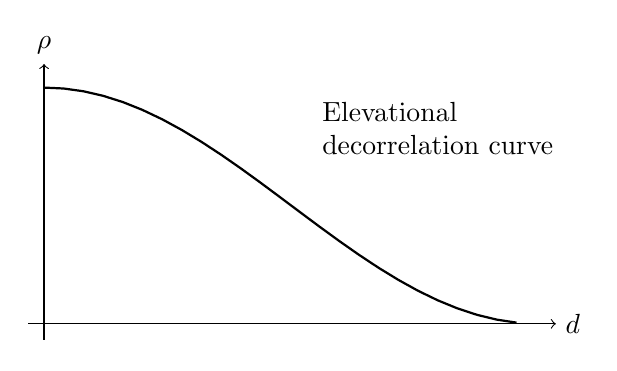
\begin{tikzpicture}[domain=0:6]
		\draw[color=black, ->] (-0.2,0) -- (6.5,0) node[right] {$d$};
		\draw[color=black, ->] (0,-0.2) -- (0,3.3) node[above] {$\rho$};
		
		% TikZ does not have a sinc function build-in, so fake it with cos
		\draw[color=black, thick] plot (\x, {1.5 * (cos(0.5 * \x r) + 1)}) node[above, xshift=-1cm, yshift=2cm, align=left] {Elevational \\ decorrelation curve};
	\end{tikzpicture}
	\caption{
		\textbf{Elevational decorrelation curve} describing the distance between two adjacent ultrasound frames given their correlation $\rho$ \cite{Housden07,Chen97,Afsham14}.
	}
	\label{fig:uscompounding:correlation-curve}
\end{figure}

Technically, the elevational decorrelation curve describing the distance $d$ of two frames given a correlation $\rho$ is of non-linear form (cf. Fig. \ref{fig:uscompounding:correlation-curve}) and needs to be carefully calibrated to the used ultrasound transducer \cite{Housden07,Chen97,Afsham14}.
However, since we assume to have tracking information available, we do not need to solely rely on speckle decorrelation and can approximate the elevational speckle curve by a linear function, which allows for a generic formulation.
For two tracked ultrasound frames $i, j$ with centroids $c_i, c_j$, we consider their correlation to be zero if their Euclidean distance exceeds a threshold $d_\text{max}$, while their correlation should be maximal if $c_i = c_j$.
Therefore, we define
\begin{equation}
	\label{eq:uscompounding:distance-term}
	D(i, j) := \max \left( \frac{d_\text{max} - \|c_i - c_j\|}{d_\text{max}} , \ 0 \right),
\end{equation}
which normalizes the correlation to the interval of $[0, 1]$.
A value of 1mm for $d_\text{max}$ showed excellent results for all our experiments.
While yielding comparable results for standard cases, this distance-based correlation term is not only simpler than the original Gaussian window formulation in \cite{Schultezub14}, but also a more robust generalization since it does also allow for non-homogeneous frame sampling rates.

We model the orientation-based correlation between two ultrasound frames by the cosine distance of their normals.
Thus, for two tracked ultrasound frames $i, j$ with normals $n_i, n_j$, we define the orientation-based correlation term as
\begin{equation}
	\label{eq:uscompounding:cosine-similarity}
	O(i, j) := \max \left( 1 - \frac{2}{\pi} \cdot \text{acos} \left( \frac{n_i \cdot n_j}{\|n_i\| \|n_j\|} \right) , \ 0 \right),
\end{equation}
which is a simple extension of the Euclidean dot product formula, normalized to yield results in the interval of $[0, 1]$.
In both terms, the maximum function avoids negative correlations.


\section{Orientation-driven Inter-frame Registration of Ultrasound Sweeps}
\label{sec:uscompounding:pressure-comp}

\begin{figure}[ht]
	\centering
	\subfloat[]{
		\label{fig:uscompounding:phantom_pressure_original}
		\includegraphics[height=5.5cm]{figures/uscompounding/phantom_pressure_original.jpg}
	}
	\subfloat[]{
		\label{fig:uscompounding:phantom_pressure_compensated}
		\includegraphics[height=5.5cm]{figures/uscompounding/phantom_pressure_compensated.jpg}
	}
	\subfloat[]{
		\label{fig:uscompounding:phantom_no_pressure}
		\includegraphics[height=5.5cm]{figures/uscompounding/phantom_no_pressure.jpg}
	}
	\caption{Reconstruction of an \textbf{abdominal phantom scan with probe pressure changes}: (a) MPR through the compounded volume without applying our pressure compensation technique; (b) the same MPR through the compounded volume with pressure compensation applied. For comparison, (c) shows the same target acquired using constant probe pressure.}
	\label{fig:uscompounding:comparison-pressure}
\end{figure}

To correct for errors and inaccuracies in the tracking data (e.g. due to jitter, inaccurate calibration or patient movement), we use the above framework for performing an intensity-based inter-frame registration, similar to Treece et al. \cite{Treece02}.
% Similar to Treece et al. \cite{Treece02}, we perform an intensity-based registration between adjacent ultrasound frames.
Since the image changes are minimal for adjacent ultrasound frames in a sweep, a simple and thus real-time capable pixel-wise uphill search evaluating the SSD is sufficient for registering each ultrasound frame to its surrounding frames in terms of in-plane translation and in-plane rotation.
To effectively compensate for registration drift, we regularize  by registering each ultrasound frame to a window of $N$ surrounding frames.
Thus, for a given reference patch $P$ and equally sized moving patch $P'$ the windowed SSD (wSSD) is given by
\begin{equation}
	\label{eq:uscompounding:wssd}
	\text{wSSD}_{P, P', N} (i) = \sum_{
		\substack{(p, p') \\ \in P \times P'}
	} \sum_{n = -N}^{N}  C(i, i+n) \cdot \big( I_i(p) - I_{i+n}(p') \big)^2,
\end{equation}
where $i$ is the index of the reference frame and $I_i(p)$ denotes the image intensity of ultrasound frame $i$ at the position $p$.


The central part in Eq. \ref{eq:uscompounding:wssd} is the correlation term $C(i, j)$, which describes the correlation between frames $i$ and $j$ and weights the surrounding frames' contribution to the similarity measure.
As motivated in the previous section, the correlation between the two frames depends on both their proximity and their orientation to each other.
Therefore, we define the $C(i, j)$ as
\begin{equation}
	\label{eq:uscompounding:correlation-term}
	C(i,j) := D(i,j) \cdot O(i,j).
\end{equation}

To compensate for probe pressure artifacts, we apply the above inter-frame registration technique not only to a single patch, but to a grid of independent patches of $10\text{mm} \times 10\text{mm}$ size.
We make the simplified assumption that for our applications a deformation model is sufficient, which expects the deformation to be only in transducer direction. 
Therefore, we allow in-plane translations of the individual patches.
After computing the transformation for each patch as above, we regularize the deformation field using a Gaussian  convolution, which corresponds to one iteration of a fluid-type demons registration \cite{Nielsen96,Thirion98,Zikic11} on the abovementioned grid.
We compute the coarse inverse deformation field using fixed-point iteration \cite{Chen08}, which is eventually extended to pixel level using bilinear filtering during the compounding process.
A exemplary result is displayed in Fig. \ref{fig:uscompounding:comparison-pressure}.



\section{An Information-fusion Approach to Ultrasound Compounding}
\label{sec:uscompounding:clustering}

Compounding ultrasound frames acquired from different viewpoints is non-trivial since ultrasound may show different intensities for the same anatomy if it is scanned from a different angle or at a different time.
This is due to the complex ultrasound image formation being dependent on many different factors such as view angle, probe pressure, patient position and breathing cycle.
Thus, tortuous acquisition sweeps are particularly challenging to reconstruct since their frames overlap.
Traditional compounding schemes based on averaging or distance-based weighting fail in correctly reconstructing such regions as illustrated in Fig. \ref{fig:uscompounding:different_angles_artifacts}.
Since closer pixels are preferred over pixels being farther away, the compounded voxel intensity mainly depends on the ultrasound frame of highest proximity.
If we now consider a neighbor voxel, the closest frame may have a completely different orientation and thus show different information (due to the view dependency of ultrasound).
The resulting reconstructions exibit a low image quality with significant discontinuities in the anatomy.
Furthermore, unwanted stripe or pixel artifacts may arise as depicted in Fig. \ref{fig:uscompounding:stripe-artifacts}. 

Besides promoting artifacts and inhomogenities, distance-based weighting can also lead to incorrect reconstruction results since the distance of the frame to the voxel has no correlation with the amount of information present in this pixel (i.e. level of uncertainty/noise).
For instance, it may ignore a pixel being farther away but having low uncertainty and instead prefer a high uncertainty pixel (i.e. noise) because it is closer to the voxel.

These two issues are the main motivation for our proposed orientation-driven ultrasound compounding technique.
It tackles them by partitioning the ultrasound sweep into clusters of similar alignment and then using additional uncertainty information in a two-step fusion approach.
We assume that for each ultrasound pixel with intensity $I_i$, we also have an uncertainty value $u_i$ that we will use for weighting the image intensities during compounding.
While our method considers the generation of uncertainty information as black box and is thus independent from it, we use for our implementation the Confidence Maps as proposed by Karamalis et al. \cite{Karamalis12}.
Even though they model ultrasound physics only to a limited amount, their Confidence Maps can be interpreted as uncertainty information. 

\begin{figure}[t]
	\centering
	\resizebox{0.75\linewidth}{!}{
		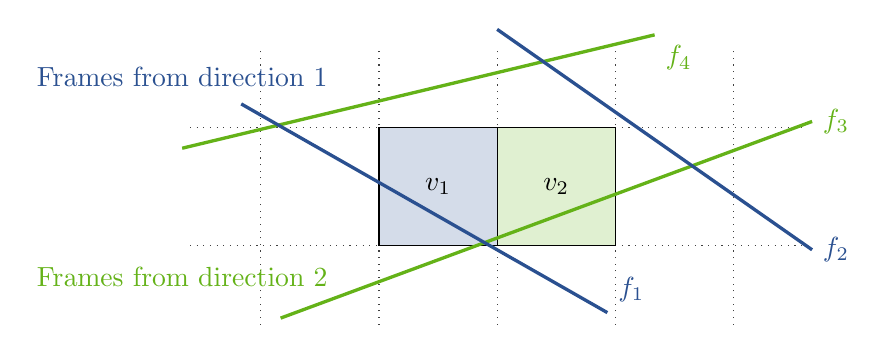
\begin{tikzpicture}[
	vertexlabel/.style={outer sep=6pt, fill=white},
	endpoint/.style={color=tumblue!75},
	midpoint/.style={color=tumblue!40},
	cluster1/.style={dagreen, very thick},
	cluster2/.style={tumblue, very thick}
	]
		\definecolor{dagreen}{RGB}{100, 178, 24}	
		\definecolor{tumblue}{RGB}{42, 80, 144}	
% 	\coordinate [label={[vertexlabel]below:{$v_0 = (x_0, y_0, z_0)$}}] (v0) at (-1.65, -2.2);
% 	\coordinate [label={[vertexlabel]above left:{$v_1 = (x_1, y_1, z_1)$}}]  (v1) at (-2.60,  0.9);
% 	\coordinate [label={[vertexlabel]below right:{$v_2 = (x_2, y_2, z_2)$}}] (v2) at ( 2.60, -0.9);
% 	\coordinate [label={[vertexlabel]above:{$v_3 = (x_3, y_3, z_3)$}}] (v3) at ( 1.65,  2.2);

	% grid
	\draw[step=1.5cm, darkgray,dotted, thin] (-3.9, -1.0) grid (3.9, 2.5);
		
	% voxel 1
	\filldraw [fill=tumblue!20] (-1.5, 0) rectangle (0, 1.5);
	\node at (-0.75, 0.75) {$v_1$};
	
	% voxel 2
	\filldraw [fill=dagreen!20] (0, 0) rectangle (1.5, 1.5);
	\node at (0.75, 0.75) {$v_2$};
	
	% Frames cluster 1
	\node [cluster1] at (-4, -0.4) {Frames from direction 2};
	\draw [cluster1, domain=-2.75:4] plot (\x, {0.37*\x + 0.1}) node[right] {$f_3$};
	\draw [cluster1, domain=-4:2.0] plot (\x, {0.24*\x + 2.2}) node[below right] {$f_4$};
	
	% Frames cluster 2
	\node [cluster2] at (-4, 2.15) {Frames from direction 1};
	\draw [cluster2, domain=-3.25:1.4] plot (\x, {-0.57*\x - 0.05}) node[above right] {$f_1$};
	\draw [cluster2, domain=-0.0:4.00] plot (\x, {-0.7*\x + 2.75}) node[right] {$f_2$};
\end{tikzpicture}

	}
	\caption{
		Illustration of \textbf{artifacts occurring in distance-weighted compounded regions} where multiple ultrasound frames from different directions intersect.
		With traditional methods, voxel $v_1$ is mainly based on the information of frame $f_1$ while its neigbour voxel $v_2$ is mainly based on the information in frame $f_3$.
			However, their intensities at this spatial location may significantly differ since the frames travel through different acoustic windows.
	}
	\label{fig:uscompounding:different_angles_artifacts}
\end{figure}

\begin{figure}[ht]
	\centering
	\subfloat[]{
		\includegraphics[width=0.95\textwidth]{figures/uscompounding/cluster-bs.jpg}
		\label{fig:uscompounding:stripe-artifacts}
	}
	\\
	\subfloat[]{
		\includegraphics[width=0.95\textwidth]{figures/uscompounding/cluster-od.jpg}
	}
	\caption{
		Effect of the \textbf{orientation-driven clustering} of ultrasound frames:
		Both images show reconstructions of a tortuous sweep of upper arm ultrasound.
		(a) Traditional techniques with distance-only weighting show severe stripe artifacts (yellow arrows) in regions of overlapping frames.
		(b) Partitioning the sweep into clusters of homogeneous orientation and fusing the clusters based on uncertainty suppreses these artifacts almost entirely.
		Please mind that both volumes were compounded \emph{without} applying our pressure compensation technique to highlight the beneficial effect of the orientation-driven clustering.
	}
	\label{fig:uscompounding:comparison-clustering}
\end{figure}

\subsection{Clustering of Ultrasound Sweeps by Direction}
As a first step, we perform a hierarchical clustering to identify tortuous sweep trajectories and regions of overlapping ultrasound frames.
This partitions the ultrasound sweep trajectory into parts where the frames have homogeneous orientation without requiring us to predefine the number of clusters.
We apply an average group linkage algorithm on the previously defined orientation term $O(i, j)$ (cf. Eq. \ref{eq:uscompounding:cosine-similarity}).
This yields a set $C$ of sub-sweeps meeting the usual restriction of being contiguous and uniformly oriented.

\subsection{Compounding of each Cluster}
\label{sec:uscompounding:compounding-of-each-cluster}
A backward warping algorithm then compounds each cluster $c \in C$ into a 3D volume $I_c$ applying our pressure compensation method as discussed in Section \ref{sec:uscompounding:pressure-comp}.
Since the ultrasound frames of each cluster are guaranteed to have the same orientation and are thus travelling through the same acoustic window, we can safely assume the uncertainty distribution to be homogeneous within nearby frames.
We compute the intensity for voxel $x$ as
\begin{equation}
	I_c(x)		=		\frac{\sum_{i\in S} I_i \cdot d_i^{-\mu}}{\sum_{i \in S} d_i^{-\mu}},
\end{equation}
where $S$ is the set of frame pixels close to the compounded voxel $x$, $d_i$ the Euclidean distance of pixel $i$ to the compounded voxel, and $\mu>1$ a smoothness parameter ensuring that $I_c(x)$ approximates the original data for $d_i \rightarrow 0$ \cite{Shepard68}.
Wein et al. showed that this inverse distance weighting scheme yields excellent results in terms of image quality \cite{Wein06}.
We use the same weighting to propagate the uncertainty to a separate 3D volume $U_c$:
\begin{equation}
	U_c(x)		=		\frac{\sum_{i\in S} u_i \cdot d_i^{-\mu}}{\sum_{i \in S} d_i^{-\mu}}.
\end{equation}

Thus, for each cluster $c \in C$ we end up with a compounded ultrasound intensity volume $I_c$ and a compounded uncertainty volume $U_c$.


\subsection{Uncertainty-based Fusion of the Compounded Clusters}
% Since ultrasound image formation is a highly non-linear process and the pixel-based uncertainty values $u_i$ are relative to the image content and thus not necessarily comparable between different frames, we perform the uncertainty-based fusion in a second step to avoid artifacts such as the ones depicted in Fig. \ref{fig:uscompounding:stripe-artifacts}.
In a final step, our method fuses the clusters together into the final 3D volume based on the propagated uncertainty values.
We want the individual clusters $c \in C$ to contribute in an additive manner weighted by the propagated voxel uncertainties.
Therefore, we compute the final intensity $I$ at voxel $x$ by
\begin{equation}
	\label{eq:uscompounding:fusion}
	I(x)		=		\frac{\sum_{c\in C} (1 - U_c(x)) I_c(x)}{\sum_{c \in C} 1 - U_c(x)}.
\end{equation}

Since we are acquiring a continuous sweep of ultrasound frames and apply a regularized inter-frame registration with active pressure compensation, we can safely assume that the individual clusters are well aligned.
Hence, an additional 3D-3D registration is not needed.


\section{Incremental Compounding System}
For interventional usage, one does not only require short processing times, but also wants to support an interactive update of the compounded volume during the acquisition to allow for an additional refinement of selected regions.
Therefore, we introduce \emph{incremental ultrasound compounding} as a real-time capable extension of our orientation-driven compounding technique.

\subsection{Incremental Compounding Pipeline}
As illustrated in Fig. \ref{fig:uscompounding:schematic-diagram}, our system receives a constant stream of incoming ultrasound frames.
The regularized inter-frame registration (cf. Section \ref{sec:uscompounding:pressure-comp}) needs only a limited number of frames lookahead (i.e. size of the regularization window) and can hence be performed on-line requiring only a small number of frames to be buffered.
We extend the orientation-driven clustering approach (cf. Section \ref{sec:uscompounding:clustering}) to a partitioning into batches of ultrasound frames.
In addition to starting new clusters when the correlation term exceeds the threshold, we also start new batches in a regular time interval (e.g. every second) to keep their size small.


Instead of reconstructing a separate volume for each batch, we use a single volume as accumulation buffer and adapt the above technique to an in-place algorithm.
The reconstructed voxels of each cluster can be incrementally added to an accumulation buffer by rewriting Eq. \ref{eq:uscompounding:fusion} to a recurrence scheme. 
Given the accumulated compounded intensity $I_{i-1}$ and accumulated compounded uncertainty $U_{i-1}$ of the previous runs, and $I_c, U_c$ of the current run, we define the new intensity $I_i$ and uncertainty $U_i$ as
\begin{equation}
	\label{eq:uscompounding:incremental-fusion}
	\begin{split}
		I_i		&=		\frac{U_{i-1} I_{i-1}   +   (1 - U_c) I_c}{U_{i-1}   +  (1 - U_c)}, \\
		U_i		&=		U_{i-1}   +  (1 - U_c).
	\end{split}
\end{equation}
This transforms our technique into an on-line algorithm, significantly lowering the computational complexity and memory footprint and furthermore allowing for an interactive update of the visualization after each batch.

Apart from a slightly worse (but in our case neglectable) numerical stability, Eq. \ref{eq:uscompounding:fusion} and Eq. \ref{eq:uscompounding:incremental-fusion} yield the same reconstruction result.
It should be noted that, with the incremental clustering, frames of the same orientation may end up in different clusters compared to the conventional formulation when they are separated by frames of different orientation.
While technically this may alter the final result, we did not observe any qualitative differences in our experiments.


\begin{figure}[ht]
	\centering
	\subfloat[No pressure compensation applied.]{
		\includegraphics[width=0.31\textwidth]{figures/uscompounding/registration0x0.jpg}
	}
	\;
	\subfloat[Inter-frame registration with $3 \times 4$ patches yielding a patch size of $10\text{mm} \times 10.5\text{mm}$.]{
		\includegraphics[width=0.31\textwidth]{figures/uscompounding/registration3x3.jpg}
	}
	\;
	\subfloat[Inter-frame registration with $4 \times 20$ patches yielding a patch size of $7.5\text{mm} \times 2.1\text{mm}$.]{
		\includegraphics[width=0.31\textwidth]{figures/uscompounding/registration5x16.jpg}
	}
	\caption{
		Multi-planar reconstructions of in-vivo acquisitions of the Infraspinatus muscle showing the \textbf{effectiveness of the pressure compensation}.
		Though the sweep was acquired by a professional sonographer trying to maintain constant probe pressure, the result of a traditional compounding technique (a) has an unsteady appearance and shows discontinuities throughout the different muscle layers.
		Applying our orientation-driven inter-frame registration and pressure compensation even on low resolution grid with $10\text{mm} \times 10.5\text{mm}$ patch size (b) yields a significant increase in image quality.
		Further increasing the resolution of the deformation field to $7.5\text{mm} \times 2.1\text{mm}$ patch size (c) yields only slight improvements.
	}
	\label{fig:uscompounding:comparison-registration}
\end{figure}

\subsection{Real-time Implementation}
The most time-consuming part of our reconstruction pipeline is the incremental compounding of each batch of ultrasound frames into the target volume.
To yield high quality results, we employ a backward compounding technique where each voxel of the target volume is compared to each ultrasound frame to find contributing pixels (cf. Section \ref{sec:uscompounding:compounding-of-each-cluster}).
This process can be parallelized heavily on voxel level.
To exploit the new features of recent graphics hardware, we implemented the entire incremental compounding process on the GPU using OpenGL 4.3.
To this end, we store the tracking information as well as other required data in Shader Storage Buffer Objects \cite{OpenGL43,SSBO} and the image data of the ultrasound frames in 2D texture arrays to support hardware-accelerated interpolation during sampling.
This allows us to yield highly interactive frame rates for the compounding process.
This is further accelerated by exploiting that we do not need to traverse the voxels of the entire target volume but can restrict the reconstruction volume of each pass to the bounding box of the corresponding batch of ultrasound frames.
Our information fusion approach exploiting uncertainty information ensures that the additional partitioning of the ultrasound sweep into batches does not impair the reconstruction quality.


\section{Results and Evaluation}
To evaluate our methods, we used an Acuson S2000\texttrademark~ultrasound machine equipped with an Acuson 9L4 linear transducer and Ascension trakSTAR\texttrademark 2 electromagnetic tracking hardware.
The system was calibrated using the method described in \cite{Wein08}, yielding an experimental calibration error of less than 2mm and 4 degrees.
We acquired both phantom and in-vivo data of different anatomies where the in-vivo sweeps were acquired by a professional sonographer.
All baseline results for comparison within this section were computed using our own implementation of a state-of-the-art backward compounding technique with inverse distance weighting as proposed by Wein et al. \cite{Wein06}.


\subsection{Parameter Evaluation}
To evaluate the effectiveness of our orientation-driven inter-frame registration and pressure compensation, and its dependency on parameters, we applied our technique to different ultrasound sweeps of both phantom and in-vivo data.
Figures \ref{fig:uscompounding:comparison-pressure} and \ref{fig:uscompounding:comparison-registration} show representative results.

All experiments show a significant improvement in terms of image appearance and continuity of anatomy features when applying inter-frame registration, even with only minimal pressure changes present in the input data.
In particular, the in-vivo scans show good results already with low resolution deformation fields, such as $3 \times 4$ patches for the Infraspinatus data set resulting in a patch size of roughly $10\text{mm} \times 10\text{mm}$.
Increasing the deformation field resolution by decreasing the patch size yields only marginal improvements while increasing the computational burden (cf Fig. \ref{fig:uscompounding:comparison-registration}).
Hence, in our implementation, we use a target patch size of $10\text{mm} \times 10\text{mm}$ as default setting.



\subsection{Reconstruction Accuracy}
To validate the physically correct reconstruction of anatomy, we acquired ultrasound sweeps of an abdominal phantom including a tumor target of spherical shape as depicted in Fig. \ref{fig:uscompounding:comparison-pressure}.
Since the target is positioned relatively close to the surface, it can be scanned from different directions and is prone to deformation.
Therefore, this is a relevant scenario to evaluate our method.
We computed 50 MPRs of arbitrary orientation through the target and compared the maximum diameter with reference measurements acquired from CT. 
The reconstructed ultrasound volume yielded an average target diameter of $14.63 \pm 0.48$ mm  compared to $14.5 \pm 0.84$ mm in CT.
This proves an excellent physical accuracy of our reconstruction method.



\subsection{Reconstruction Quality}
The qualitative effects of our inter-frame registration and pressure compensation technique can be observed in Fig. \ref{fig:uscompounding:comparison-pressure} and \ref{fig:uscompounding:comparison-registration} showing the reconstructions of different ultrasound sweeps. 
The originally round target of the abdominal phantom (Fig. \ref{fig:uscompounding:phantom_no_pressure}) is severely deformed through probe pressure changes (Fig. \ref{fig:uscompounding:phantom_pressure_original}).
Our pressure compensation technique is capable of mostly restoring the original anatomy (Fig. \ref{fig:uscompounding:phantom_pressure_compensated}).
While the original shape is not perfectly restored, there is a clear improvement visible.
Also Fig. \ref{fig:uscompounding:comparison-registration} shows significant improvements in terms of continuity of anatomy when enabling our pressure compensation.
Compared to \cite{Treece02}, there is still room for improvement. 
However, we want to emphasize that the implemented pressure compensation is of only complementary nature and the focus of this work is die orientation-driven clustering and compounding technique.

Fig. \ref{fig:uscompounding:comparison-clustering} demonstrates the effect of our clustering technique when reconstructing a twisted ultrasound sweep of a human arm exhibiting out-of-plane rotations of up to 35 degrees.
Due to overlapping frames, the standard compounding in (a) shows artifacts at locations where the frames for neighboring voxels are acquired through different acoustic windows.
The reconstruction in (b) removes such artifacts by using our clustering technique to avoid overlapping frames in a single cluster. 
Additionally, it exploits uncertainty information when fusing the clusters so that unreliable intensities do not bias the final result.
Please note that, in order to highlight the effect of the clustering, these volumes were reconstructed without  pressure compensation and thus show discontinuities in the anatomy.

\begin{figure}[ht]
	\centering
	\includegraphics[width=0.75\textwidth]{figures/uscompounding/achilles_3d.jpg}
	
	\caption{
			\textbf{3D visualization of an achilles tendon} data set compounded with our technique.
			Due to the high curvature of the skin surface this is a challenging anatomy for sonography.
			Our clinical partners appreciate the high quality spatial reconstruction where possible lesions are easy to identify.
	}
	\label{fig:uscompounding:achilles-3d}
\end{figure}

To further illustrate a clinical application, Fig. \ref{fig:uscompounding:achilles-3d} shows a 3D visualization of an achilles tendon ultrasound volume acquired with our technique.
Due to the high curvature of the surrounding skin surface, this is a challenging anatomy for ultrasound compounding.
Our clinical partners highly appreciate the reconstruction quality where they can easily identify possible lesions in a spatial context.

To quantitatively evaluate the effectiveness of our orientation-driven compounding technique in terms of ensuring continuity of the anatomy and reducing artifacts in regions of overlapping ultrasound frames, we evaluate a local, scale-invariant entropy measure of the reconstructed sweeps.
For every voxel we computed the intensity difference to the neighboring voxels and computed the mean and standard deviation over the entire volume.
This measure penalizes high frequency intensity changes such as the mentioned stripe artifacts while preferring smooth and continuous reconstructions of the anatomy, which are desired for clinical and visualization purposes.
To avoid biasing the result, we considered only the inner part of the volume and masked the outer faces of the sweep, as they naturally have a high entropy.
The results as displayed in Table \ref{tbl:entropy} show that our technique is sucessful in reducing the amount of reconstruction artifacts.
While the entropy measures are not directly comparable between the data sets, all test data sets with a twisted probe trajectory show a significant drop in the mean difference and standard deviation.
As reference, the first line shows the measure for a data set with a strictly linear sweep trajectory.
Here, the drop in entropy turns out to be much lower.



\begin{table}[th]
	\centering
	\caption{		
			Quantification of the local entropy in compounded volumes in terms of mean intensity difference to neighboring voxels.
	}
	\label{tbl:entropy}
	\begin{tabu} to 0.95\linewidth {>{\bfseries\centering}m{55mm} C C}
		\toprule
		\                                & \bfseries Baseline \cite{Wein06} & \bfseries Our Technique \\
		\midrule
		In-vivo leg / linear sweep       & $2.65 \pm 2.42$                  & $2.49 \pm 2.39$         \\
		\midrule
		In-vivo arm	/ twisted sweep      & $4.59 \pm 8.42$                  & $2.44 \pm 4.62$         \\
		In-vivo leg	/ twisted sweep      & $3.58 \pm 5.82$                  & $2.34 \pm 4.19$         \\
		In-vivo carotid artery	/ twisted & $7.2 \pm 13.35$                  & $3.17 \pm 8.58$         \\
		In-vivo infraspinatus	/ twisted  & $4.17 \pm 7.21$                  & $2.99 \pm 6.17$         \\
		\bottomrule
	\end{tabu}
\end{table}

\begin{figure}[ht]
	\centering
	\subfloat[Baseline]{
		\label{fig:uscompounding:msd_baseline}
		\includegraphics[width=0.48\textwidth]{figures/uscompounding/difference2_baseline.png}
	}
	\subfloat[Our Technique]{
		\label{fig:uscompounding:msd_ours}
		\includegraphics[width=0.48\textwidth]{figures/uscompounding/difference2_ours.png}
	}
	\caption{
		\textbf{Illustration of our evaluation method}: First two images show the MPRs for each perpendicular sweep, the third one shows the color-coded absolute difference of their intensities after 3D-3D rigid registration.
		(a) traditional backward-compounding \cite{Wein06} fails to align the different structures; 
		(b) our technique yields alignment of all structures.
		The quantitative results are shown in Table \ref{tbl:registration-results}.
	}
	\label{fig:uscompounding:comparison-msd}
\end{figure}

For further quantitative evaluation we acquired pairs of overlapping sweeps with perpendicular main trajectory.
After compounding the sweeps into separate 3D volumes using our methods, we applied a 3D-3D rigid registration using the tracking data as initialization.
Expecting our techniques to yield better matching volumes, we compared the differences of the two volumes in the overlapping region.
With the average of the two volumes as expected result for a correct reconstruction, we quantify their difference in Normalized Cross-Correlation (NCC) and log-scale Signal to Noise Ratio (SNR\textsubscript{dB}), for which define the signal as average of the volumes and the noise as RMS of the differences (Table \ref{tbl:registration-results}).

\begin{table}[th]
	\centering
	\caption{NCC and log-scale SNR in the overlapping region after registering the two compounded volumes of two sweeps with perpendicular trajectories of the same anatomy.}
	\label{tbl:registration-results}
	\begin{tabu} to 0.95\linewidth {>{\bfseries\centering}m{55mm} CC CC}
		\toprule
		\quad                          & \multicolumn{2}{c}{\bfseries Baseline \cite{Wein06}} & \multicolumn{2}{c}{\bfseries Our technique} \\
		\quad                          & NCC    &        SNR\textsubscript{dB}        & NCC    &  SNR\textsubscript{dB}   \\
		\midrule
		Phantom / constant pressure    & $0.90$ &               $19.39$               & $0.94$ &         $23.16$          \\
		Phantom / pressure changes     & $0.81$ &               $13.02$               & $0.94$ &         $22.47$          \\
		\midrule
		In-vivo leg / constant changes & $0.72$ &               $ 9.21$               & $0.76$ &         $11.69$          \\
		In-vivo leg / pressure changes & $0.67$ &               $ 8.53$               & $0.75$ &         $11.03$          \\
		\bottomrule
	\end{tabu}
\end{table}

The sweeps with pressure changes show a significant improvement in terms of increase in both NCC and SNR\textsubscript{dB} when our technique is applied.
Furthermore, when comparing constant pressure with pressure changes, our technique shows significantly less drop of the measures.
The slight improvements for the sweeps acquired with constant pressure are mainly due to the inter-frame registration correcting for the tracking error.
Since the sweeps are acquired with perpendicular trajectories and the volumes therefore show different interpretations of the underlying data, no algorithm yields a perfect match.
Furthermore, the in-vivo sweeps are expected to have lower similarity since they show by far less homogeneous anatomy.
Figure \ref{fig:uscompounding:comparison-msd} shows the difference images for the second phantom sweep.




\subsection{System Performance}
For the evaluation of the system performance, we ran our implementation on a workstation with an Intel Core\texttrademark~ i7-4770 CPU and a nVidia GeForce\texttrademark~ GTX 670 GPU.
We loaded recordings of different ultrasound acquisitions, streamed them into our incremental compounding pipeline and measured the time required for computing the final reconstructed volume at different resolutions. 

\begin{table}[th]
	\centering
	\caption{
		System performance of our incremental compounding technique at different target volume resolutions.
		The timings measure the compounding only (no generation of uncertainty information or visualization).
	}
	\label{tbl:performance}
	\begin{tabu} to 0.95\linewidth {m{2mm}m{32mm} C C C}
		\toprule
		& \bfseries Voxel Size		& \bfseries Volume Size										& \bfseries Time					& \bfseries Speed \\
		\midrule
		\multicolumn{2}{l}{\bfseries In-vivo arm} & & & \\ %\multicolumn{3}{c}{\addd{500 frames}} \\
		& $0.5$ mm			& $160 \times 119 \times 157$		& 728 ms 				& 687 fps \\
		& $0.25$ mm			& $320 \times 237 \times 313$		& 1551 ms				& 322 fps \\
		& $0.1$ mm			& $800 \times 591 \times 781$		& 13499 ms			& 37 fps \\
		\midrule
		\multicolumn{2}{l}{\bfseries In-vivo leg} & & & \\ %\multicolumn{3}{c}{\addd{241 frames}} \\
		& $0.5$ mm			& $187 \times 138 \times 101$		& 389 ms				& 620 fps \\
		& $0.25$ mm			& $373 \times 276 \times 214$		& 906 ms				& 266 fps \\
		& $0.1$ mm			& $931 \times 689 \times 533$		& 8433 ms			  & 29 fps \\
		\midrule
		\multicolumn{2}{l}{\bfseries In-vivo carotid artery} & & & \\ %\multicolumn{3}{c}{\addd{488frames}} \\
		& $0.5$ mm			& $90 \times 62 \times 97$			& 657 ms 				& 743 fps \\
		& $0.25$ mm			& $179 \times 124 \times 194$		& 735 ms				& 664 fps \\
		& $0.1$ mm			& $447 \times 308 \times 485$		& 2569 ms				& 189 fps \\
		\midrule
		\multicolumn{2}{l}{\bfseries In-vivo infraspinatus} & & & \\ %\multicolumn{3}{c}{\addd{370 frames}} \\
		& $0.5$ mm			& $114 \times 104 \times 178$		& 609 ms 				& 608 fps \\
		& $0.25$ mm			& $228 \times 207 \times 355$		& 1135 ms				& 326 fps \\
		& $0.1$ mm			& $570 \times 517 \times 887$		& 6761 ms				& 55 fps \\
		\bottomrule
	\end{tabu}
\end{table}

Table \ref{tbl:performance} shows the timings for four exemplary data sets.
The performance mainly depends on the number of frame pixels contributing to a single voxel (i.e. relationship between pixel size, voxel size and frame sampling rate) as well as the number of identified clusters (i.e. tortuosity of the sweep).
The results show that for a clinically adequate resolution of $0.25$ mm voxel size, our system has enough bandwidth to reconstruct ultrasound sweeps of very high framerate.
Even high-quality reconstructions of $0.1$ mm voxel size can be compounded at interactive frame rates.


\section{Conclusion}
In this work, we presented a novel orientation-driven approach featuring an incremental compounding scheme. 
We developed our methods with the aim to free clinicians from the restrictive scanning protocols of many of today's state of the art methods, which require the acquisition of linear probe trajectories and constant probe pressure.
Our target application within this work was MSK ultrasound, where typical sweeps exhibit pressure changes, back- and forth and twisting motion.
Therefore, we introduced a framework of two correlation terms to capture that the correlation of two frames in an ultrasound sweep depends on their proximity and orientation to each other.
This framework is used to perform a complementary pressure compensation as well as a clustering of ultrasound frames by orientation to remove different kinds of artifacts.
In the subsequent compounding process, we use an information fusion approach exploiting ultrasound Confidence Maps.
This allows for more accurate reconstructions in regions where we have information from different acoustic windows, since intensities from uncertain regions do not bias intensity information from reliable regions.
Finally, we presented an integrated system for incremental compounding that interactively fills the reconstructed volume while acquiring the sweep.
This provides the clinician with direct feedback on the ongoing acquisition and allows for an interactive refinement of target regions.


We evaluated the different aspects of our technique using both phantom and in-vivo data, which was acquired by a professional sonographer.
The results show that our methods accurately reconstruct the original anatomy and yield superior results than traditional backward compounding methods in terms of image quality, continuity of the anatomy and presence of artifacts.
Furthermore, the evaluation of our integrated incremental compounding system shows that the proposed system has enough bandwidth to reconstruct ultrasound sweeps with more than a hundred frames per second when using a clinically adequate target voxel size of 0.25mm.
Even with high resolution volumes of 0.1mm voxel size, we still can yield interactive frame rates to update the compounded volume during the acquisition.

Hence, we see our orientation-driven approach as an important step towards providing clinicians with more freedom regarding 3D freehand ultrasound scanning protocols so that they can focus on which images the acquire instead of on how they have to acquire them.
Current limitations of our work are mostly formed by the rather simple pressure compensation, which is not always capable of fully undoing all deformations.
Therefore, as further work, we would like to merge more sophisticated pressure compensation techniques, such as \cite{Treece02}, into our orientation-driven framework.

t
%\cleardoublepage

%\part{Personal Pointing Interaction}
%% !TEX root = ../thesis-example.tex
%
\chapter{Calibration and Recovery of Personal Pointing Gesture}
\label{chap:3-PAST}
%why the topic is coming to important 
It is widely believed that as the computing,communication, and display technologies progress further, the existing user interaction solution may become a bottleneck for the effective interaction with desired information. 
Today, we are facing more and more digital information controlled by different computing devices.
Selection is the first and one of the important steps in the natural user interaction process as the computing device has to know which object the user is interested in. In most cases, the user is aware of where and what the information is but can't directly begin interaction since time is lost to make the corresponding computing device know where the desired information is\cite{Swindells2002}. 
For example, different information can be shown in multiple displays, however, the user will have a problem interacting with the information if the displays are not within reach. In addition, computers can understand the ambient scenario via object detection or 3D reconstruction, but the user can't directly perform interaction with the desired object or tell the computers how to understand the 3D volume\cite{export:244725}.
Hence, designing better natural user interfaces is still an vital concern.

The pointing gesture is fundamental to human behavior \cite{Matthews2012} and used consistently across cultures \cite{McNeill2000}. It begins at an early developmental stage \cite{Carpendale2010} and lets humans  reference proximal objects as well as abstract concepts in the world. It is also natively combined with hand gestures. Pointing gestures, which are part of our gestural language, are inherently used for interaction\cite{Nanayakkara2013a}. Only a few works try to model and estimate the user{\rq}s pointing geometry when performing interaction with ambient information.One existing technique consists in positioning a camera next to the monitor or display and observing the user. In this case, the computing device can understand the user{\rq}s pointing behavior by detecting the user{\rq}s gaze. Unfortunately, the user has to stand within a limited working zone defined by the targeted display and the camera, as shown in \figurename{ \ref{fig:3-PAST:problem}(a)}.
Other inventors have taken advantage of wearable cameras enabling the user to perform interaction with digital information\cite{Harrison2011} \cite{Mistry2009}.
These works detect the user's finger and calculate the pointing geometry from the camera view instead of the user's eye, as shown in \figurename{ \ref{fig:3-PAST:problem}(b)}. This setup works well when the user performs interaction with information which should is reachable.
%The camera view still could replace the user view when a visual hint was display or the user's view is controlled.
However, \figurename{ \ref{fig:3-PAST:problem}(c)} illustrates an important problem when the user equipped with a wearable camera tries to point at objects which are not reachable. There is a significant offset between $O_{eye}$, the object which is pointed towards in the user's view, and $O_{camera}$, the object in the camera's view. 
\begin{figure} [htb]
	\centering
	\includegraphics[width= 1.0\linewidth]{figures/3-PAST/problem.png}
	\caption{(a)There is a limited working zone, when positioning a camera next to the monitor or display while observing the user.(b)The user's view could be replaced by the camera view when the desired object is reachable. (c) There is a significant offset when the user points at a not reachable object.}
	\label{fig:3-PAST:problem}
\end{figure}
Wearable vision systems have potential ability to acquire contextual information through computer vision techniques\cite{Kurata2000}. Usually, the wearable device calibration is not possible and often scale, rotation, and/or translation-invariant features are required in higher level modules. If the wearable device could understand the user{\rq}s pointing geometry, then the pointing gesture will augment the capabilities of the wearable device by enabling a multi-point control 3D interface in a mixed reality (MR) setting. Here we aim at developing  an ubiquitous solution allowing the wearable device to always understand the spatial relationship between the user{\rq}s specific pointing gesture and the ambient information within the mixed reality world.

\section{PAST Methodology}
\label{sec:3-PAST:Methodology}
we propose a method that facilitates a wearable device calibration of a user's pointing gesture in order to model and recover the user specific pointing geometry. The pointing geometry is modeled as a line of sight, which starts from a virtual eye center and goes through the fingertip to the desired target information. During the calibration process, the user is asked to perform pointing gestures towards several targets shown to them. A user specific virtual eye center is then estimated based on the detected fingertip.
This process enables to accurately determine where the user is pointing at in a mixed reality environment. This work is different than the current methods for hand gesture recognition and gesture based interaction.  Its main difference lies within a novel concept and method for calibrating and recovering the pointing geometry with a user's specific habit, enabling direct interaction with real and virtual digital elements of interest within the user's environment.

\subsection{General Design}
\label{sec:3-PAST:GD}
In a general hardware design, the wearable device should be put on the user's head and contain two sensors, $S_{f}$ and $S_{c}$. The  $S_f$ is used to detect the fingertip which the user uses to perform the pointing gesture and calculate its 3D position. The $S_c$ goes to acquire the contextual information of the objects in front of the user. In general, the  $S_f$ should provide a near-range depth map as the 3D position of the fingertip has to be accurately calculated. The contextual information should be acquired with 3D position as the pointing gesture is performed in the 3D world.The $S_c$ could be a color camera, a depth sensor or a RGB-D sensor in different scenarios to acquire a known object with 3D position or a valid depth map of the real world. The $S_c$ could also be calibrated related to a head mounted display (HMD) to acquire the contextual information of the virtual world. As $S_c$ and  $S_f$ are just different types of camera, the self calibration of the wearable device could be performed using Zhang{\rq}s method \cite{Zhang2000}.

\subsection{Pointing At Several Targets (PAST)} \label{sec:3-PAST:PAST}
As a human, both eyes perceive a stereo view and the images are processed by our brains to generate the 3D scene of the objects in front of us. We always perceive a unified 3D scene no matter how we rotate our eyes. In other words, there should be a fixed original point of the 3D scene in our brain and here we define it as the virtual eye center. When performing pointing gestures, a user could always directly put their fingertips somewhere between their eyes and the target to generate a line of sight, which goes through the fingertip and the target. Thus we model the pointing geometry as a line, which starts from the virtual eye center and goes through the fingertip and the target, as shown in \figurename{ \ref{fig:3-PAST:PSATCalibration}}. It is important to emphasize that the virtual eye center is not the middle point between the user's eyes. As discussed in Section \ref{sec:3-PAST:results}, users may be left or right eye dominant which affects the location of the virtual eye center. Fortunately, the PAST method accounts for this.

%Inspired by the Single-Point Active Alignment Method (SPAAM) for Optical See-Through head mounted display calibration for augmented reality \cite{Tuceryan2000},
The objective of \textbf{Pointing At Several Targets (PAST)} method is to calibrate and recover the specific pointing geometry. The result of the calibration is the position of a virtual eye center $E$ for the user. Based on the pointing model, we could collect a set of pointing lines and estimate the intersection to finish the calibration.
As shown in \figurename{ \ref{fig:3-PAST:PSATCalibration}}, the target ,$T_i$, is shown somewhere at the front of the user, who is asked to perform a pointing gesture towards $T_i$ using one finger naturally. The 3D positions of the fingertips $F_i$ and $T_i$ are collected through $S_f$ and $S_c$, respectively. The pointing line $L_i$ ,which passes through $F_i$ and $T_i$, would also go through $E$ . After enough pointing lines are collected, the intersection of the lines should be $E$. After calibration, the user specific virtual eye-center $E$ is known and the pointing geometry would be recovered as $L_{i}$, going through $E$ and  $F_i$, when the pointing gesture is performed.
\begin{figure} [htb]
	\centering
	\includegraphics[width= \linewidth]{figures/3-PAST/Calibration.png}
	\caption{Calibration of the user specific pointing gesture: the user is asked to point at several targets using one finger and the pointing lines which pass through $F_i$ and $T_i$ are collected. The intersection of these lines should be $E$, the user specific virtual eye-center.}
	\label{fig:3-PAST:PSATCalibration}
\end{figure}

\subsection{Target the user points at} \label{sec:3-PAST:findTarget}
As defined in section \ref{sec:3-PAST:GD}, the contextual information always could be expressed in a 3D world and a mesh surface could be generated accordingly. 
Based on the PAST method, the user specific pointing geometry could be recovered as the pointing line $L_{i}$, going through $E$ and  $F_i$, when the pointing gesture is performed.
As shown in \figurename{ \ref{fig:3-PAST:pointToTarget}} , a $Mesh$ surface is generated based on the contextual information. The intersection between $L_{i}$ and $Mesh$ is $T_i$, the target which the user points at. 
\begin{figure} [htb]
	\centering
	\includegraphics[width= \linewidth]{figures/3-PAST/pointToTarget.png}
	\caption{ The intersection between the pointing line $L_{i}$ and the $Mesh$ is  $T_i$, the 3D position of the target or information the user points at.}
	\label{fig:3-PAST:pointToTarget}
\end{figure}

We propose an example scenario where the user is equipped with a wearable RGB-D sensor to perform a pointing gesture interaction with information shown on a display.
The depth sensor generates a near-range depth map and acts as $S_f$, and the color camera as $S_c$ acquires the contextual information. The 3D position of a fingertip could be calculated from a valid depth map when the pointing gesture is performed. It is very easy to detect a display and compute its plane function using image features. As the targets are shown on the display, the 3D contextual information of the display and the targets are acquired using the color camera. The calibration of the RGB-D sensor is performed using Zhang{\rq}s method \cite{Zhang2000}. During the PAST calibration, the targets are shown on the display and the user is asked to perform pointing gesture towards the targets (see Section \ref{sec:3-PAST:PAST}). After calibration, the pointing line $L_i$ is calculated and the  $Mesh$ is generated from the plane function of the display. According to \figurename{ \ref{fig:3-PAST:pointToTarget}}, the intersection between the pointing line $L_{i}$ and $Mesh$ is  $T_i$, the 3D position of the target or information shown on the display the user is pointing at.

\section{Feasibility Analysis of PAST} \label{sec:3-PAST:FA}
The pointing gesture is fundamental to human behavior and is also quite personal \cite{Matthews2012}. If the images in the user's eyes were accessible, then $F_i$ , the fingertip detected in $S_f$, and $E$, the eye center calculated in PAST calibration, would be perfect. In addition, the human eyes are an auto-focus stereo camera, but can't focus on objects in different depths at the same time. In our proposed system, the user is asked to focus on the target and not on the fingertip, which allows the user to perform the pointing naturally. Thus the fingertip in the user's view is different from the one detected by $S_f$. 

As shown in \figurename{ \ref{fig:3-PAST:fingertipOffset}}, $F_i$  and $T_i$  are the fingertip and the target, which are detected by the wearable device respectively, and $E$ is the virtual eye center calculated in the PAST calibration procedure. $\bar F_i$ and $\bar T_i$ are the fingertip and target in the user{\rq}s own view, and $\bar E$ is the ideal virtual eye center. So there is a vector $V_{fi}$ from $\bar F_i$ to $F_i$, $F_i = {\bar F_i} + V_{fi}$ when the pointing is performed at all times. $T_i = {\bar T_i}$ in the calibration procedure as the user is asked to point towards a known target. $L_i$ is the pointing line estimated by the wearable device and $\bar L_i$ is the ideal pointing line in the user{\rq}s view. 
\begin{figure} [htb]
	\centering
	\includegraphics[width= \linewidth]{figures/3-PAST/fingerOffset.png}
	\caption{ Here is the pointing geometry during the calibration and recovery procedure. There is a vector $V_{fi}$  from $\bar F_i$ to $F_i$ when the pointing gesture is performed and a vector $V_{E}$, from the ideal virtual eye-center ${\bar E}$ to $E$.}
	\label{fig:3-PAST:fingertipOffset}
\end{figure}
\subsection{Calibration} \label{sec:3-PAST:PASTCalibration}
Based on the assumption of the pointing geometry model, the pointing line $\bar L_i$ is starting from $\bar E$ going through $\bar F_i$ and ending at the desired target $\bar T_i$. We could use Eq. \ref{equ:pointOnLineUser} to  represent all the points along the pointing line $\bar L_i$, and $\bar E$ is the intersection of all the pointing line $\bar L_i$. This means that there is a $\bar \lambda_i$ making both Eq.\ref{equ:lambdaLineuser} and Eq.\ref{equ:intersectionOfLineUser} true for every  $\bar L_i$.
\begin{equation}  \label{equ:pointOnLineUser}
P_{\bar L_i} = {\bar T_i} + \bar\lambda ({\bar F_i} - {\bar T_i}) ,\bar\lambda \in R 
\end{equation}
\begin{equation} \label{equ:lambdaLineuser}
\bar\lambda_i = \frac {D_{\bar E2 \bar T_i}}{D_{\bar E2 \bar T_i} -D_{\bar E2 \bar F_i}} 
\end{equation}
where $D_{\bar E2 \bar F_i}$ is the distance from $\bar E$ to ${{\bar F_i}}$ and $D_{\bar E2 \bar T_i}$ is the distance from ${\bar E}$ to ${\bar T_i}$. 
\begin{equation} \label{equ:intersectionOfLineUser}
{\bar E} = {\bar T_i} + \bar\lambda_i ({\bar F_i} - {\bar T_i}) 
\end{equation}
The pointing line detected by the wearable device is $L_i$, which goes through  ${T_i}$ and $F_i$. All the points along $L_i$ could be represented as:
\begin{equation} \label{equ:pointOnLineSensor}
P_{L_i} = {T_i} + \lambda(F_i - {T_i}) , \lambda \in R 
\end{equation}
$F_i$ in Eq. \ref{equ:pointOnLineSensor} could be replaced by ${\bar F_i} + V_{fi}$ and ${T_i} = {\bar T_i}$ during calibration. Hence,
\begin{equation} \label{equ:pointOnlineSensor2}
P_{L_i} = {\bar T_i} + \lambda({\bar F_i} - {\bar T_i}) + \lambda V_{fi}, \lambda \in R 
\end{equation}
There is a point $E_i$ on the line $P_{L_i}$, when $\lambda = \bar\lambda_i$ in Eq.\ref{equ:pointOnlineSensor2}.
\begin{equation} \label{equ:P_eye}
E_i = {\bar T_i} + \bar\lambda_i({\bar F_i} - {\bar T_i}) + \bar\lambda_i V_{fi}  
\end{equation}
After putting Eq. \ref{equ:intersectionOfLineUser} into Eq.\ref{equ:P_eye}, there is always a point $E_i$ along every $L_i$ and could be represent as:
\begin{equation} \label{equ:P_eye2}
E_i = {\bar E} + \bar\lambda_i V_{fi}  
\end{equation}
\begin{figure} [htb]
	\centering
	\includegraphics[width= \linewidth]{figures/3-PAST/lambdai.png}
	\caption{$\bar \lambda_i$ decreases as $D_{\bar E2 \bar T_i}$ increases in three different cases, but the difference is very small.}
	\label{fig:3-PAST:lambdai}
\end{figure}
%and the maximum length of  $V_{fi}$  is about the size of nail, 10 mm
When PAST calibration is performed, we could fix the $D_{\bar E2 \bar T_i}$ and $\bar \lambda_i$ is only affected by $ D_{\bar E2 \bar F_i}$. As shown in \figurename{ \ref{fig:3-PAST:lambdai}}, $\bar \lambda_i$ decreases slowly as $D_{\bar E2 \bar T_i}$ increases in three different example cases. The maximum delta of $\bar \lambda_i$ is smaller than 0.1. $\bar\lambda_i$ could be rewritten as:
\begin{equation} \label{equ:lambdai}
\bar\lambda_i = \bar\lambda_c + \Delta \bar\lambda_i
\end{equation}
where $\bar\lambda_c \in \left[1.0,1.2\right]$ is constant part and $\Delta \bar\lambda_i \in \left[0,0.1\right] $. 
$V_{fi}$ is different every time and could also be represented as $V_{fc} + {\Delta V_{fi}}$, where $V_{fc}$ is a stable offset and ${\Delta V_{fi}}$ is a small random deviation. So,
\begin{equation} \label{equ:lambdavf}
\bar\lambda_i V_{fi} \approx  \bar\lambda_c V_{fc}  + \bar\lambda_i {\Delta V_{fi}} %+ \Delta \bar\lambda_i V_{fc} + \bar\lambda_c {\Delta V_{fi}}
\end{equation}
where $\bar\lambda_c {\Delta V_{fi}} + \bar\lambda_i {\Delta V_{fi}}$ is very small.  $\bar\lambda_c V_{fc}$ is consistent, so $\delta \bar\lambda_{i} V_{fc}$ is the main contribution of the variation of $\bar\lambda_i V_{fi}$. Even when there is about 2 cm offset between $F$ and $\bar{F}$, there exist two points $E_m$ and $E_n$ along any two lines $L_m$ and $L_n$ respectively and the maximal distance between $E_m$ and $E_n$ is about 0.2 cm. There is a valid candidate point $E$, which is very close to of all the lines $L_i$. Hence, the PAST calibration is feasible and the offset between $E$ and $\bar{E}$ is approximately $ \bar\lambda_c V_{fc}$. 
\begin{equation} \label{equ:P_eyeCalib}
E \approx {\bar E} + \bar\lambda_c V_{fc} 
\end{equation} 
\subsection{Pointing geometry recovery} \label{sec:3-PAST:PASTrecovery}
As shown in \figurename{ \ref{fig:3-PAST:fingertipOffset}}, $E$ is the calibration result with an offset $V_{E} \approx \bar\lambda_c V_{fc}$, between $E$ and the ideal virtual eye-center ${\bar E}$. 
When the user points towards a target after calibration, the position of the target calculated by the wearable device, $T_i$, could be represented by $E$ and $F_i$ as:
\begin{equation} \label{equ:targetInSensor}
T_i = E+ \frac{D_{E2T_i}}{D_{E2F_i}}  \left( {F_i - E} \right)
\end{equation}
where $D_{E2F_i}$ is the distance from $E$ to ${{F_i}}$ and $D_{E2T_i}$ is the distance from ${E}$ to ${T_i}$. \\
$\bar T_i$ , the position of the ideal target in the user's view, could be expressed as:
\begin{equation} \label{equ:targetInEye}
\bar T_i \approx {\bar E} + \frac{D_{E2T_i}}{D_{E2F_i}}  \left( {{\bar F_i} - {\bar E}} \right)
\end{equation}
${\angle}_{E}$, the angle error between the user's pointing lines to $T_i$ and $\bar T_i$ could be calculated using Eq.\ref{equ:tanViewAngle} as $D_{E2T_i}$ is much larger than the offset of the target. 
\begin{equation} \label{equ:tanViewAngle}
{\angle}_{E} = \tan^{-1} \left( {\frac{| {T_i - \bar T_i}| }{D_{E2T_i}} } \right)
\end{equation}
After substituting Eq.\ref{equ:P_eyeCalib}, Eq.\ref{equ:targetInSensor} and Eq.\ref{equ:targetInEye}, we get :
\begin{equation} \label{equ:tanViewAngle1}
{\angle}_{E} \approx \tan^{-1} \left( {{\frac{{\lambda_c{|V_{fc}|} }}{D_{E2T_i}} + \frac{{|\lambda_i V_{fi} - \lambda_c V_{fc}|} }{D_{E2F_i}}} } \right)
\end{equation}
As ${\angle}_{E}$ is very small, we get after substituting Eq.\ref{equ:lambdavf}:
\begin{equation} \label{equ:ViewAngleError}
{\angle}_{E} \approx \frac{ {\lambda_c{|V_{fc}|}} }{D_{E2T_i}} + \frac{ {|\Delta \bar \lambda_i V_{fc}|} }{D_{E2F_i}}
\end{equation}
\begin{figure} [htb]
	\centering
	\includegraphics[width= \linewidth]{figures/3-PAST/EvaluationOfPointing.png}
	\caption{The angle error decreases as $D_{E2T}$ increases and $V_{fc}$ decreases. $D_{E2F}$ does not really affect the accuracy of the pointing gesture.}
	\label{fig:3-PAST:evaluatinOfPointing}
\end{figure}
As shown in \figurename{ \ref{fig:3-PAST:evaluatinOfPointing}}, the angle error decreases as $V_{fc}$ decreases and $D_{E2T_i}$ increases. $D_{E2Fi}$ does not really affect the accuracy of the recovered pointing gesture. The accuracy of recovered pointing line is below 0.9\degree.

Based on the above feasibility analysis we can conclude that the PAST method recovers a user specific virtual eye center which enables the wearable device to determine where the user points at accurately.

\section{Evaluation \& Results}
\subsection{Implementation}
In this part, we implement the example scenario described in section \ref{sec:3-PAST:findTarget}, where the user is equipped with a wearable RGB-D device to perform interaction with a display using pointing gesture.
\paragraph{Hardware}
Intel{\rq}s \textit{RealSense} 3D sensor  was selected to act as the wearable RGB-D device, which contains a 640x480 depth sensor (Valid Range:0.2-1.2 meters) and a 1920x1080 color camera. The depth sensor $S_f$ is used to detect the fingertip  and the color camera $S_c$ to acquire 3D contextual information. The \textit{RealSense} 3D sensor is strapped on the user{\rq}s head using a bandana with an adjusted height and angle (see \figurename{ \ref{fig:3-PAST:hardWare}}). 
A 46$''$ TV display and a 24$''$ monitor were positioned around the user with various information displayed on the screens as the contextual environment. 
%new finger with a raised finger TODO: retake a pircure of the hardware setup
\begin{figure}[htb]
	\centering
	\includegraphics[width = \linewidth]{figures/3-PAST/hardWare.png}
	\caption{The side and front view of the wearable device setup. The \textit{RealSense} 3D sensor is strapped on the user{\rq}s head using a bandana.}
	\label{fig:3-PAST:hardWare}
\end{figure}
\paragraph{Fingertip detection}
%The depth sensor and the color camera are packaged in one device and observe at the same direction. This resulted in not obtaining good contextual information and finger depth maps simultaneously. 
The near range depth sensor could generate a real-time depth image of the hand or finger when the user performs pointing gesture. The fingertip detection technology in \cite{Betancourt2015} was not employed as there was no full depth map of the hand. Hand and finger blobs were directly extracted from the depth image using the \textit{Intel RealSense SDK} and the contours and the convex hull were calculated using the method provided by \cite{Suzuki1985}. Then, the best peak was chosen as the detected fingertip. 
%\textcolor{red}{the following paragraph is not very clear}
%For each fingertip defect, there are 3 points: two peaks and the defect, as shown in \figurename{ \ref{fig:tips}} . We detect a fingertip in the first peak if the angle between the two peaks and the defect is lower than 90\degree and if the norm in pixel is higher than 15.
%\begin{figure} [h]
%	\centering
%	\includegraphics[width=1.5in]{./../images/tips.jpg}
%	\caption {  We detect a fingertip in the first peak if the angle between the two peaks and the defect is lower than 90\degree and if the norm in pixel is higher than 15.}
%	\label{fig:tips}
%\end{figure}
\paragraph{Contextual Information} {\label{sec:3-PAST:markerDetection}}
To simplify the task to acquire the contextual information, we used the \textit{ARTooKitPlus}\cite{Wagner2007a} library to detect the TV display and monitor. There were two implementations: A) Some markers were directly shown  on screen only if it did not affect the current information shown on the screen. The markers instead of the screen were detected to calculate the 3D contextual information. B) Physical printed markers were put next to the display and others were shown on the screen and then a calibration was done to calculate the transformation matrix from the printed markers to the screen. During the user study, the wearable device detected the printed markers and calculated the position of the screen to acquire the contextual information. As shown in \figurename{ \ref{fig:3-PAST:MarkerTracking}}, the screen was detected using method A during the PAST calibration and evaluation and method B was employed during the ``PictureView" demo.
\begin{figure}[htb]
	\centering
	\includegraphics[width = \linewidth]{figures/3-PAST/display.png}
	\caption{(1) Four \textit{ARTooKitPlus} markers shown on the dispaly, (2) A target shown during the PAST calibration, (3) The ``PictureView" demo, (4) A printed \textit{ARTooKitPlus} marker. Left: During the PAST calibration, the screen was detected via the screen marker. Right: A printed marker was tracking during the ``PictureView" demo.}
	\label{fig:3-PAST:MarkerTracking}
\end{figure}
%todo: detection finger tip from two hand at the same time 
%	 how to describe the algorithm to simulate the mouse click 
%	 simple drawing demo using two hands at the same time
\paragraph{PictureView Demo} \label{sec:3-PAST:pictureviewDemo}
In this section, a ``PictureView" demo was developed using the pointing gesture to perform interaction. Several pictures were shown on the screen and the user was asked to select the picture and move it to a defined location, as shown in \figurename{ \ref{fig:3-PAST:MarkerTracking}}. After PAST calibration, the user could directly perform pointing gesture towards the screen to manipulate the picture as the wearable device could recover the pointing geometry and understand the spatial relationship between the pointing gesture and the pictures shown on the display. The selection command was recognized when the user pushed the fingertip along the pointing line. After selection, the picture was moved along the user's pointing gesture. When the picture was moved to the right area, the picture was dissociated with the pointing gesture and disappeared. Or the picture was also dissociated and reset to original position when moved to wrong area. See the supplementary video accompanying this paper.

\subsection{User Study Design}
%questions: do we have to keep the first bared-hand cablibration 
To understand the performance and system usability of the PAST method, we conducted some quantitative and qualitative evaluations. For the user study, we designed several tasks in different scenarios and the participants were asked to finish all these tasks. Lastly the users answered a questionnaire to evaluate the ``PictureView" demo.
\paragraph{Scenario for Experiments}
The TV display and the monitor were placed in front of the user. The participant firstly put the wearable RGB-D device on their heads and adjusted the height and angle to make sure that the color camera has a full view of the display in front of them, while ensuring the depth sensor has a valid depth map of the fingertip when they performed pointing gesture in a comfortable pose. There were three kinds of tasks for the user to do during the user study:
\begin{enumerate} [label= (\Alph*)]%[(a)] ,leftmargin=*
	%Evaluation of Calibration method: time consuming and error
	\item \label{task:calib} Calibration: A red target was shown at several different position on the TV display and the user was asked to perform pointing gesture towards the red target using one finger. 
	%The data is automatically collected when the user hold the finger still for one second.
	\item \label{task:pointEvaluation}Evaluation: A blue target was shown at several different position on the TV or the monitor and the user was asked to perform pointing gesture towards the blue target using one finger.
	\item \label{task:PointWithFeedback}Evaluation with visual feedback: A blue target was shown at some different position one the TV. The user performed pointing gesture towards the display with a green point shown as a visual feedback. The user was asked to match the green point and the blue target as close as possible. 
\end{enumerate}
\paragraph{Study Description}
\textbf{Participants}
Ten people (6 Male and 4 Female, and Age Range: 22-34) from different cultures were enrolled in the user study. Three of them were born and brought up in Germany, three in China, two in Chile, one in France and one in India. Seven of them had a degree of computer science. Nine were reported to be right-handed, while one was ambidextrous.

\textbf{Study procedure} Before starting the user study, participants were supervised to perform the pointing in the proposed pose to make sure the wearable device could detect the markers and the fingertip accurately at the same time. The user was asked to focus on the target not the fingertip when performing pointing. After a simple training session, participants were asked to do the following 10 steps to evaluate the proposed method and system.
\begin{enumerate}%[(1)]
	\item \label{step:stereoCalib} Do task \ref{task:calib} three times from 2 meters away to finish PAST calibration and evaluate if the calibration was stable. The first calibration result is employed for all the following evaluation.
	\item \label{step:pointWithFeedback} Do task \ref{task:PointWithFeedback} on the TV display from 2 meters away to give the participant an intuitive feeling of this technology, check the calibration result, and evaluate if the visual feedback would improve the accuracy and precision.
	\item \label{step:pointingEvaluation} Do task \ref{task:pointEvaluation} on the TV display from 2 meters away to evaluate the accuracy and precision of the recovered pointing geometry.
	\item \label{step:diffentHand} Do task \ref{task:pointEvaluation} on the TV display using another hand from 2 meters away to evaluate if the PAST calibration was independent of the finger.
	%one calibration: test with different hand and finger
	\item \label{step:distanceEvaluation} Redo task \ref{task:pointEvaluation} on the TV display from 1.5,3 and 4  meters away, to evaluate the accuracy of the recovered pointing geometry at different distances.
	\item \label{step:differentScreenEvaluation}  Do task \ref{task:pointEvaluation} on the monitor from 2 meters away to evaluate if the calibration is independent of the display.
	\item \label{step:calibDifferentDistance} Redo task \ref{task:calib} three times from 1.5, 3 and 4 meters away to evaluate if the calibration is independent of the target distance. 
	\item \label{step:calibOneEye} Redo task \ref{task:calib} with only left or right eye open from 2 meters away to understand the relationship of the two eyes and the calculated virtual eye center. 
	\item \label{step:pictureview} Play with the demo ``PicureView" for 2 minutes using the first calibration result calculated in step \ref{step:stereoCalib} to evaluate the system usability,.
	\item \label{step:questionnaire} The interpupillary distance of the participant was measured with a ruler and the user completed a questionnaire to evaluate the system.
\end{enumerate}

\subsection{Results} \label{sec:3-PAST:results}
%diagrams and analyze the collected data
The real interpupillary distance of the ten participants was measured in step \ref{step:questionnaire} and was distributed from 6.0 to 6.8cm. In step \ref{step:calibOneEye}, the left and right eye were calibrated related to the wearable device and the interpupillary distance was subsequently calibrated. Compared to the true measured distance from step 10, the average distance between eyes is $0.11\pm0.11$ cm. From this, we conclude that the PAST method could accurately measure the user's eye center. 

From step \ref{step:stereoCalib} and \ref{step:calibOneEye}, we could get the positions of the left, right and virtual eye-center related to the wearable device. When all interpupillary distances were upscaled to 7 cm, the spatial relationship of the left, right and virtual eye-center can be seen in \figurename{ \ref{fig:3-PAST:virtualEye}}. 
The position of the virtual eye-center was very user specific and influenced by the user specific pointing gesture. As such, we could not simply take the left eye, right eye, or middle point between the user's eyes as the virtual eye center to recover the pointing geometry. Hence, the PAST calibration is necessary to recover an accurate pointing geometry.
\begin{figure}[htb] 
	\centering
	\includegraphics[width=\linewidth]{figures/3-PAST/virtualEye.png}
	\caption{As three points are coplanar, the spatial relationship was shown in a 2D coordinate system. The middle point of the two eyes was set as the original center and the spatial relationship of the left, right and the calculated virtual eye-center is shown in green.}
	\label{fig:3-PAST:virtualEye}
\end{figure}

The average calibration results in step \ref{step:stereoCalib} was taken as the reference to evaluate if the PAST calibration was stable and independent of the distance. The 3D distances from the virtual eye calculated from 1.5, 2, 3, and 4 meters away to the reference one are $0.83\pm0.73cm$, $0.56\pm0.41cm$,$0.90\pm0.73cm$, and $1.02\pm0.72cm$, respectively. 
As shown in \figurename{ \ref{fig:3-PAST:PAST}}, the offset in the XY plane was less than 0.5 cm in most cases. The offset along the Z axis was bigger than the XY plane as the PAST method calculates the intersection of some pointing lines which pass along Z axis. 
%However the offset was still less than 1 cm in most cases.
The 3D distance calculated from 1.5 meters was greater than the one from 2 meters aways, since $\bar\lambda_i$ increases as the $ D_{\bar E2 \bar F_i}$ decreases ( as seen in section \ref{sec:3-PAST:PASTCalibration}).  
The calibrations in 3 and 4 meters were not so stable as the ones in 1.5 and 2 meters as the marker tracking was not so accurate. The four charts in \figurename{ \ref{fig:3-PAST:PAST}} show the PAST method could provide a stable calibration result for different users and the calibration was independent of the contextual environment. 

\begin{figure}[htb]
	\centering
	\includegraphics[width=\linewidth]{figures/3-PAST/PAST.png}
	\caption{The calibration results were compared to the reference one showing distribution of the offset along X,Y and Z axis. The XY plane was the one approximately parallel to the user's face. These four charts show the offset of the calibrations from different distances. (a) 1.5 meters away (b) 2 meters away (c) 3 meters away (d) 4 meters away.}
	\label{fig:3-PAST:PAST}
\end{figure}
The first PAST calibration result in step \ref{step:stereoCalib} was employed to evaluate the recovered pointing geometry in different scenarios, with and without visual feedback, with a different hand, from different distance and towards a different display. To evaluate the recovered pointing geometry, ${\angle}_{E}$ was calculated according to Eq. \ref{equ:ViewAngleError} to evaluate the accuracy. The precision was the difference of ${\angle}_{E}$ in consecutive frames while the participant performed pointing gestures to the same target. To get a clear distribution of the error of the recovered pointing lines, the vector from the $\bar T_i$ to $T_i$ was also calculated. As shown in \figurename{ \ref{fig:3-PAST:Accuracy2m}} and \figurename{ \ref{fig:3-PAST:Accuracy}}, for every point in the charts the distance to the original was the angle value in degrees and the points were distributed according to the vector from the $\bar T_i$ to $T_i$.

The pointing accuracies shown in \figurename{ \ref{fig:3-PAST:Accuracy2m}(a-c)} are $0.16\pm0.13$\degree, $0.37\pm0.28$\degree, and $0.60\pm0.73$\degree, respectively.  In \figurename{ \ref{fig:3-PAST:Accuracy2m}(b)} the ${\angle}_{E}$ of most points was less than 0.5\degree (consistent with  \figurename{ \ref{fig:3-PAST:evaluatinOfPointing}} ), so the pointing geometry was correctly recovered. Comparing \figurename{ \ref{fig:Accuracy2m}(a) and \ref{fig:3-PAST:Accuracy2m}(b)}, it was found that the visual feedback improved the accuracy as the user could adjust their pointing gesture. As seen in \figurename{ \ref{fig:3-PAST:Accuracy2m}(c)}, the calibration still worked well with another hand in most cases.The precisions of the pointing line with and without feedback were very stable and less than 0.2\degree, shown in \figurename{ \ref{fig:3-PAST:Accuracy2m}(d)}, so the wearable device could stably recover the pointing geometry.
\begin{figure} [htb]
	\centering
	\includegraphics[width=\linewidth]{figures/3-PAST/accuracy2m.png}
	\caption{After calibration, the participants performed pointing gestures towards some targets to evaluate if the pointing geometry could be correctly recovered. (a) perform pointing with feedback from 2 meters away (b) perform pointing from 2 meter aways (c) perform pointing with another hand, different with the one used for calibration (d) the precision when the participants performed pointing with and without feedback from 2 meters away.}
	\label{fig:3-PAST:Accuracy2m}
\end{figure}

The pointing accuracies shown in \figurename{ \ref{fig:3-PAST:Accuracy}(a-d)} are $0.69\pm0.84$\degree, $0.57\pm0.43$\degree, $0.79\pm0.92$\degree, and $0.64\pm0.57$\degree, respectively. As expected in \figurename{ \ref{fig:3-PAST:evaluatinOfPointing}}, the ${\angle}_{E}$ increased at 1.5 meters away in \figurename{ \ref{fig:3-PAST:Accuracy}(a)}, compared to \figurename{ \ref{fig:3-PAST:Accuracy2m}(b)}. However, \figurename{ \ref{fig:3-PAST:Accuracy}(b) and \ref{fig:3-PAST:Accuracy}(c)} show the ${\angle}_{E}$ didn't decrease when the pointing was performed from 3 and 4 meters away as the accuracy of the contextual information declined. \figurename{ \ref{fig:3-PAST:Accuracy}(d)} demonstrates that the calibration was contextually independent and the pointing geometry was still recovered with the 24$''$ monitor. 

As shown in \figurename{ \ref{fig:3-PAST:Accuracy2m}} and \figurename{ \ref{fig:3-PAST:Accuracy}}, ${\angle}_{E}$ is less than 1\degree in most cases in different scenarios and less than 0.5\degree with an accurate contextual information. The overall pointing accuracy at 1.5, 2, 3, and 4 meters is $0.60\pm0.70$\degree. We conclude that the pointing gesture was recovered accurately.
\begin{figure} [htb]
	\centering
	\includegraphics[width=\linewidth]{figures/3-PAST/accuracy.png}
	\caption{The participants performed pointing gesture towards some targets in different scenarios to evaluate if calibration was contextually independent. (a) perform pointing from 1.5 meters away (b) 3 meters away (c) 4 meters away (d) perform pointing towards the 24 in monitor }
	\label{fig:3-PAST:Accuracy}
\end{figure}

%questionnaire
A questionnaire was designed to get a qualitative evaluation about the pointing interaction and the ``PictureView" demo. A Likert scale was used which is a type of psychometric response scale often used in surveys and is the most widely used scale in survey research. When responding to a Likert questionnaire item, participants specify their level of agreement to a statement. The format of our 5-pt Likert was: (1) strongly disagree, (2) disagree, (3) neither agree nor disagree, (4) agree, (5) strongly agree.
\begin{table}
	\caption{The Likert scale results of the questionnaire}
	\label{tb:3-PAST:questionnaire}
	\scriptsize
	\begin{center}
		\begin{tabular}{p{5.5cm}|p{1.2cm}}
			Questions & Scale \\
			\hline
			\textit{Q1:}I think that I would like to use this system &  $4.0\pm0.8$ \\
			\textit{Q2:}I found the system necessarily complex & $4.7\pm0.5$ \\
			\textit{Q3:}I thought the system was easy to use & $4.2\pm0.9$ \\
			\textit{Q4:}I don't think that I would need the support of a technical person to be able to use this system & $4.1\pm1.0$\\
			\textit{Q5:}I  think the system is consistent & $4.3\pm0.6$ \\
			\textit{Q6:}I would imagine that most people would learn to use this system very quickly & $4.4\pm0.5$ \\
			\textit{Q7:}I felt very confident using the system & $4.3\pm0.6$ \\
			\textit{Q8:}I didn't need to learn a lot of things before I could get going with this system & $4.5\pm0.5$
		\end{tabular}
	\end{center}
\end{table}
As shown in table \ref{tb:3-PAST:questionnaire}, all questions attained a positive scores above 4.0. Q1 had the lowest score as some participants felt a little tired while continuously lifting their arm to perform pointing gestures. In the demo the selection command was recognized as the user pushed their fingers along the pointing line, which was a little different than with a natural click hand gesture, thus the participant required some time to get used to it. In general the participants liked the pointing interaction very much and could learn it very easily and quickly. In their opinion, the finger pointing interaction was very natural. 

\section{Discussion \& Conclusion}
PAST offers a novel concept and method for recovering the user specific pointing habits that enables direct interaction with real and virtual digital elements of interest within the user's environment. 
As seen in \figurename{ \ref{fig:3-PAST:virtualEye}}, the virtual eye center $E$ calculated by PAST is user specific. The PAST calibration is very important for recovering the user specific pointing geometry. In addition, the proposed method is contextually independent and could also be used to calculate the eye position in the wearable device coordinate system. 

As shown in our user study, the PAST method could finish calibration stably and recover the user specific pointing geometry in different scenarios, with an accuracy of less than $0.5\degree$ with an accurate contextual information and less than $1\degree$ in most cases. The participants could easily learn how to use this new interaction method. However, the gesture combined with the pointing still should be improved. In addition, the PAST calibration could be separately done for every  finger allowing the user to use multi-finger to perform a multi-control 3D interaction in a mixed reality setting. Given the recent increased interest in using speech to interact with mobile devices, it is a logical next step to support a user in pointing at an object while stating a comment or asking a question about it.

Pointing At Several Targets method facilitates the calibration of the user's pointing gesture that models and recovers the user specific pointing geometry and subsequently calculates where the user is pointing at. Mathematical analysis and experimental results demonstrate that the PAST method could model and calibrate the pointing gesture stably and recover the user specific pointing gesture correctly. The calibration method is contextually independent and in most cases the pointing line was recovered with accuracy less than $1\degree$ and less than $0.5\degree$ with accurate contextual information. The overall pointing accuracy at 1.5, 2, 3, and 4 meters is $0.60\pm0.70$\degree. The PAST solution would enable a whole series of applications in which the user may acquire or interact with digital information and opens the path towards development of new interaction paradigms: the user could directly perform multi-control 3D interaction with virtual or real elements placed within the mixed reality environment.
%\input{content/3-PointingOR}

% --------------------------
% Back matter
% --------------------------
{%
\setstretch{1.1}
\renewcommand{\bibfont}{\normalfont\small}
\setlength{\biblabelsep}{4pt}
\setlength{\bibitemsep}{0.5\baselineskip plus 0.5\baselineskip}
\printbibliography[nottype=online]
\printbibliography[heading=subbibliography,title={Online Resources},type=online,prefixnumbers={@}]
}
\cleardoublepage

%%uncomment the follow comment scope after you finish the writing.
%\listoffigures
%\cleardoublepage
%
%\listoftables
%\cleardoublepage
%
%\input{content/declaration}
\clearpage
\newpage
\mbox{}

% **************************************************
% End of Document CONTENT
% **************************************************
\end{document}
